\documentclass{ximera}  


%\usepackage{todonotes}
%\usepackage{mathtools} %% Required for wide table Curl and Greens
%\usepackage{cuted} %% Required for wide table Curl and Greens
\newcommand{\todo}{}

\usepackage{esint} % for \oiint
\ifxake%%https://math.meta.stackexchange.com/questions/9973/how-do-you-render-a-closed-surface-double-integral
\renewcommand{\oiint}{{\large\bigcirc}\kern-1.56em\iint}
\fi


\graphicspath{
  {./}
  {jpg}
  {ximeraTutorial/}
  {basicPhilosophy/}
  {functionsOfSeveralVariables/}
  {normalVectors/}
  {lagrangeMultipliers/}
  {vectorFields/}
  {greensTheorem/}
  {shapeOfThingsToCome/}
  {dotProducts/}
  {partialDerivativesAndTheGradientVector/}
  {../productAndQuotientRules/exercises/}
  {../motionAndPathsInSpace/exercises/}
  {../normalVectors/exercisesParametricPlots/}
  {../continuityOfFunctionsOfSeveralVariables/exercises/}
  {../partialDerivativesAndTheGradientVector/exercises/}
  {../directionalDerivativeAndChainRule/exercises/}
  {../commonCoordinates/exercisesCylindricalCoordinates/}
  {../commonCoordinates/exercisesSphericalCoordinates/}
  {../greensTheorem/exercisesCurlAndLineIntegrals/}
  {../greensTheorem/exercisesDivergenceAndLineIntegrals/}
  {../shapeOfThingsToCome/exercisesDivergenceTheorem/}
  {../greensTheorem/}
  {../shapeOfThingsToCome/}
  {../separableDifferentialEquations/exercises/}
  {vectorFields/}
}

\newcommand{\mooculus}{\textsf{\textbf{MOOC}\textnormal{\textsf{ULUS}}}}

\usepackage{tkz-euclide}\usepackage{tikz}
\usepackage{tikz-cd}
\usetikzlibrary{arrows}
\tikzset{>=stealth,commutative diagrams/.cd,
  arrow style=tikz,diagrams={>=stealth}} %% cool arrow head
\tikzset{shorten <>/.style={ shorten >=#1, shorten <=#1 } } %% allows shorter vectors

\usetikzlibrary{backgrounds} %% for boxes around graphs
\usetikzlibrary{shapes,positioning}  %% Clouds and stars
\usetikzlibrary{matrix} %% for matrix
\usepgfplotslibrary{polar} %% for polar plots
\usepgfplotslibrary{fillbetween} %% to shade area between curves in TikZ
\usetkzobj{all}
\usepackage[makeroom]{cancel} %% for strike outs
%\usepackage{mathtools} %% for pretty underbrace % Breaks Ximera
%\usepackage{multicol}
\usepackage{pgffor} %% required for integral for loops



%% http://tex.stackexchange.com/questions/66490/drawing-a-tikz-arc-specifying-the-center
%% Draws beach ball
\tikzset{pics/carc/.style args={#1:#2:#3}{code={\draw[pic actions] (#1:#3) arc(#1:#2:#3);}}}



\usepackage{array}
\setlength{\extrarowheight}{+.1cm}
\newdimen\digitwidth
\settowidth\digitwidth{9}
\def\divrule#1#2{
\noalign{\moveright#1\digitwidth
\vbox{\hrule width#2\digitwidth}}}





\newcommand{\RR}{\mathbb R}
\newcommand{\R}{\mathbb R}
\newcommand{\N}{\mathbb N}
\newcommand{\Z}{\mathbb Z}

\newcommand{\sagemath}{\textsf{SageMath}}


%\renewcommand{\d}{\,d\!}
\renewcommand{\d}{\mathop{}\!d}
\newcommand{\dd}[2][]{\frac{\d #1}{\d #2}}
\newcommand{\pp}[2][]{\frac{\partial #1}{\partial #2}}
\renewcommand{\l}{\ell}
\newcommand{\ddx}{\frac{d}{\d x}}

\newcommand{\zeroOverZero}{\ensuremath{\boldsymbol{\tfrac{0}{0}}}}
\newcommand{\inftyOverInfty}{\ensuremath{\boldsymbol{\tfrac{\infty}{\infty}}}}
\newcommand{\zeroOverInfty}{\ensuremath{\boldsymbol{\tfrac{0}{\infty}}}}
\newcommand{\zeroTimesInfty}{\ensuremath{\small\boldsymbol{0\cdot \infty}}}
\newcommand{\inftyMinusInfty}{\ensuremath{\small\boldsymbol{\infty - \infty}}}
\newcommand{\oneToInfty}{\ensuremath{\boldsymbol{1^\infty}}}
\newcommand{\zeroToZero}{\ensuremath{\boldsymbol{0^0}}}
\newcommand{\inftyToZero}{\ensuremath{\boldsymbol{\infty^0}}}



\newcommand{\numOverZero}{\ensuremath{\boldsymbol{\tfrac{\#}{0}}}}
\newcommand{\dfn}{\textbf}
%\newcommand{\unit}{\,\mathrm}
\newcommand{\unit}{\mathop{}\!\mathrm}
\newcommand{\eval}[1]{\bigg[ #1 \bigg]}
\newcommand{\seq}[1]{\left( #1 \right)}
\renewcommand{\epsilon}{\varepsilon}
\renewcommand{\phi}{\varphi}


\renewcommand{\iff}{\Leftrightarrow}

\DeclareMathOperator{\arccot}{arccot}
\DeclareMathOperator{\arcsec}{arcsec}
\DeclareMathOperator{\arccsc}{arccsc}
\DeclareMathOperator{\si}{Si}
\DeclareMathOperator{\scal}{scal}
\DeclareMathOperator{\sign}{sign}


%% \newcommand{\tightoverset}[2]{% for arrow vec
%%   \mathop{#2}\limits^{\vbox to -.5ex{\kern-0.75ex\hbox{$#1$}\vss}}}
\newcommand{\arrowvec}[1]{{\overset{\rightharpoonup}{#1}}}
%\renewcommand{\vec}[1]{\arrowvec{\mathbf{#1}}}
\renewcommand{\vec}[1]{{\overset{\boldsymbol{\rightharpoonup}}{\mathbf{#1}}}\hspace{0in}}

\newcommand{\point}[1]{\left(#1\right)} %this allows \vector{ to be changed to \vector{ with a quick find and replace
\newcommand{\pt}[1]{\mathbf{#1}} %this allows \vec{ to be changed to \vec{ with a quick find and replace
\newcommand{\Lim}[2]{\lim_{\point{#1} \to \point{#2}}} %Bart, I changed this to point since I want to use it.  It runs through both of the exercise and exerciseE files in limits section, which is why it was in each document to start with.

\DeclareMathOperator{\proj}{\mathbf{proj}}
\newcommand{\veci}{{\boldsymbol{\hat{\imath}}}}
\newcommand{\vecj}{{\boldsymbol{\hat{\jmath}}}}
\newcommand{\veck}{{\boldsymbol{\hat{k}}}}
\newcommand{\vecl}{\vec{\boldsymbol{\l}}}
\newcommand{\uvec}[1]{\mathbf{\hat{#1}}}
\newcommand{\utan}{\mathbf{\hat{t}}}
\newcommand{\unormal}{\mathbf{\hat{n}}}
\newcommand{\ubinormal}{\mathbf{\hat{b}}}

\newcommand{\dotp}{\bullet}
\newcommand{\cross}{\boldsymbol\times}
\newcommand{\grad}{\boldsymbol\nabla}
\newcommand{\divergence}{\grad\dotp}
\newcommand{\curl}{\grad\cross}
%\DeclareMathOperator{\divergence}{divergence}
%\DeclareMathOperator{\curl}[1]{\grad\cross #1}
\newcommand{\lto}{\mathop{\longrightarrow\,}\limits}

\renewcommand{\bar}{\overline}

\colorlet{textColor}{black}
\colorlet{background}{white}
\colorlet{penColor}{blue!50!black} % Color of a curve in a plot
\colorlet{penColor2}{red!50!black}% Color of a curve in a plot
\colorlet{penColor3}{red!50!blue} % Color of a curve in a plot
\colorlet{penColor4}{green!50!black} % Color of a curve in a plot
\colorlet{penColor5}{orange!80!black} % Color of a curve in a plot
\colorlet{penColor6}{yellow!70!black} % Color of a curve in a plot
\colorlet{fill1}{penColor!20} % Color of fill in a plot
\colorlet{fill2}{penColor2!20} % Color of fill in a plot
\colorlet{fillp}{fill1} % Color of positive area
\colorlet{filln}{penColor2!20} % Color of negative area
\colorlet{fill3}{penColor3!20} % Fill
\colorlet{fill4}{penColor4!20} % Fill
\colorlet{fill5}{penColor5!20} % Fill
\colorlet{gridColor}{gray!50} % Color of grid in a plot

\newcommand{\surfaceColor}{violet}
\newcommand{\surfaceColorTwo}{redyellow}
\newcommand{\sliceColor}{greenyellow}




\pgfmathdeclarefunction{gauss}{2}{% gives gaussian
  \pgfmathparse{1/(#2*sqrt(2*pi))*exp(-((x-#1)^2)/(2*#2^2))}%
}


%%%%%%%%%%%%%
%% Vectors
%%%%%%%%%%%%%

%% Simple horiz vectors
\renewcommand{\vector}[1]{\left\langle #1\right\rangle}


%% %% Complex Horiz Vectors with angle brackets
%% \makeatletter
%% \renewcommand{\vector}[2][ , ]{\left\langle%
%%   \def\nextitem{\def\nextitem{#1}}%
%%   \@for \el:=#2\do{\nextitem\el}\right\rangle%
%% }
%% \makeatother

%% %% Vertical Vectors
%% \def\vector#1{\begin{bmatrix}\vecListA#1,,\end{bmatrix}}
%% \def\vecListA#1,{\if,#1,\else #1\cr \expandafter \vecListA \fi}

%%%%%%%%%%%%%
%% End of vectors
%%%%%%%%%%%%%

%\newcommand{\fullwidth}{}
%\newcommand{\normalwidth}{}



%% makes a snazzy t-chart for evaluating functions
%\newenvironment{tchart}{\rowcolors{2}{}{background!90!textColor}\array}{\endarray}

%%This is to help with formatting on future title pages.
\newenvironment{sectionOutcomes}{}{}



%% Flowchart stuff
%\tikzstyle{startstop} = [rectangle, rounded corners, minimum width=3cm, minimum height=1cm,text centered, draw=black]
%\tikzstyle{question} = [rectangle, minimum width=3cm, minimum height=1cm, text centered, draw=black]
%\tikzstyle{decision} = [trapezium, trapezium left angle=70, trapezium right angle=110, minimum width=3cm, minimum height=1cm, text centered, draw=black]
%\tikzstyle{question} = [rectangle, rounded corners, minimum width=3cm, minimum height=1cm,text centered, draw=black]
%\tikzstyle{process} = [rectangle, minimum width=3cm, minimum height=1cm, text centered, draw=black]
%\tikzstyle{decision} = [trapezium, trapezium left angle=70, trapezium right angle=110, minimum width=3cm, minimum height=1cm, text centered, draw=black]




 
\title{Impedance Matching} 
\author{Milica Markovic} 
\outcome{Design impedance matching circuits.}
\begin{document}  
\begin{abstract}  

\end{abstract}  
\maketitle    

\section{Power}

The current and voltage phasor transformation is defined as

\begin{eqnarray}
v(t)=\Re\{|V|e^{j\theta_v} e^{j \omega t}\} \\
i(t)=\Re\{|I|e^{j\theta_i} e^{j \omega t}\}
\end{eqnarray}

Where $|V|e^{j\theta_v}$ and $|I|e^{j\theta_i}$ are phasors of voltage and current, and usually denoted with a tilde $\tilde{}$ over capital letters  $\tilde{V}$, $\tilde{I}$.


\begin{eqnarray}
v(t)=\Re\{\tilde{V} e^{j \omega t}\} \\
i(t)=\Re\{\tilde{I} e^{j \omega t}\}
\end{eqnarray}


The real part of a complex number can also be found as $\Re\{z\}=\frac{1}{2}(z +z^*)$, so the above two equations can be re-written as

\begin{eqnarray}
v(t)=\frac{1}{2} ( \tilde{V}e^{j \omega t} + \tilde{V}^*e^{-j \omega t} ) \label{phasorV}\\
i(t)=\frac{1}{2} ( \tilde{I}e^{j \omega t} + \tilde{I}^*e^{-j \omega t} ) \label{phasorI}\\
\end{eqnarray}

The power is defined as a product of voltage in current.

\begin{equation}
p(t) = v(t) i(t)
\end{equation}

If we replace voltage and current in the time domain with Eq \ref{phasorV} and \ref{phasorI} we get



\begin{eqnarray}
p(t) =\frac{1}{4} ( \tilde{V}e^{j \omega t} + \tilde{V}^*e^{-j \omega t} ) ( \tilde{I}e^{j \omega t} + \tilde{I}^*e^{-j \omega t} ) \\
p(t)=\frac{1}{4} (\tilde{V}\tilde{I}^*+ (\tilde{V}\tilde{I}^*)^*+ \tilde{V}\tilde{I}^* e^{2j \omega t}+ (\tilde{V}\tilde{I}^* e^{2j \omega t})^*)
\end{eqnarray}

We can again apply equation $\Re\{z\}=\frac{1}{2}(z +z^*)$ to simplify the above equation to

\begin{eqnarray}
p(t)=\frac{1}{2} (\Re\{\tilde{V}\tilde{I}^*\}+ \Re\{\tilde{V}\tilde{I} e^{2j \omega t }\})
\end{eqnarray}

This can also be re-written as

\begin{eqnarray}
p(t)=\frac{1}{2} \Re\{ |V| e^{j\theta_v} |I| e^{-j\theta_i} \}+ \frac{1}{2} \Re\{|V| e^{j\theta_v} |I| e^{j\theta_i} e^{2j \omega t }\} \\
p(t)=\frac{1}{2} \Re\{ |V| |I| e^{j(\theta_v-\theta_i)} \}+ \frac{1}{2} \Re\{|V| |I|  e^{j(\theta_v+\theta_i)}  e^{2j \omega t }\}
\end{eqnarray}


p(t) above is instantaneous power, $S=\tilde{V}\tilde{I}^*=|V| |I| e^{j(\theta_v-\theta_i)}$ is complex power. Complex power has real and reactive parts S=P+jQ. The first part of the equation represents the average real power P delivered to the load $P=\frac{1}{2}\Re\{\tilde{V}\tilde{I}^*\}$, and the second part represents the fluxtuating power. We are usually interested in the average real power P delivered to the load.

To find the real power delivered to the load, one would take the real part of the complex power. If we know that the impedance of the load is $Z=R+jX$, the voltage is $ \tilde{V} = Z \tilde{I}$ and we remember that $\tilde{I} \tilde{I}^* = |I|^2$ then the real power is

\begin{eqnarray}
P=\frac{1}{2}\Re\{ \tilde{V} \tilde{I}^*  \} \\
P=\frac{1}{2}\Re\{ (R+jX) \tilde{I} \tilde{I}^*  \} \\
P=\frac{1}{2}\Re\{ (R+jX) |I|^2  \} \\
P=\frac{1}{2}|I|^2 \Re\{ (R+jX)   \} \\
P=\frac{1}{2}R |I|^2 
\end{eqnarray}




\begin{example}
A transmitter operated at 20MHz, Vg=100V with $50 \Omega$ internal impedance is connected to an antenna load through 6.33m of the line. The line is a lossless $50 \Omega$, $\beta=0.595rad/m$. The antenna impedance at 20MHz measures $Z_L=36+j20 \Omega$. 
\begin{enumerate}
\item What is the electrical length of the line? (answer: length=0.6$\lambda$)
\item How much power is delivered to the line? Hint: Find the input impedance, then find the input power as $P_{ave,in}=\frac{1}{2}R_{in} |I_{in}|^2$
\item What is the time-average power absorbed by $Z_L$. $P_{L}=\frac{1}{2} R_L |I_{L}|^2$
\item If now we match load impedance $Z_l$ to 50 Ohm line, what is the input impedance of the line, and how much average power is delivered to the line and load?
\end{enumerate}

\end{example}


\subsection*{Power Transfer on a Transmission Line}

Power on a transmission line can be found similarly to the derivation in the previous section. It is just that now, the total voltage is the sum of the forward going and reflected voltage, and the total current is the sum of the forward and reflected current. 


\begin{eqnarray}
\tilde{V}(z)=\tilde{V}_0^+ e^{-\gamma z} + \tilde{V}_0^- e^{\gamma z}\label{eq4a} \\
I(z)=\tilde{I}_0^+ e^{-\gamma z} + \tilde{I}_0^- e^{\gamma z}\label{eq5a}
\end{eqnarray}

Where $\tilde{V}^+(z)=\tilde{V}_0^+ e^{-\gamma z} $ is the phasor of forward voltage anywhere on the line, and $\tilde{V}^-(z)=\tilde{V}_0^- e^{\gamma z}$ is the phasor of reflected voltage anywhere on the line. $\tilde{V}_0^+$ is the phasor of forward voltage at the load, where z=0, and  $\tilde{V}_0^-$ is the phasor of reflected voltage at the load, where z=0.  The currents are similarly named. If the line is lossless, then the attenuation coefficient $\alpha=0$ and $\gamma= \alpha + j \beta = j \beta$, so the equations become



\begin{eqnarray}
\tilde{V}(z)=\tilde{V}_0^+ e^{-j\beta z} + \tilde{V}_0^- e^{j\beta z}\label{eq4} \\
I(z)=\tilde{I}_0^+ e^{-j\beta z} + \tilde{I}_0^- e^{j\beta z}\label{eq5}
\end{eqnarray}

If we define a phasor of reflection coefficient at the load as $\Gamma =\frac{\tilde{V}^-_0(z)}{\tilde{V}^+_0(z)}$, and define the transmission-line impedance as $Z_0=\frac{\tilde{V}_0^+}{\tilde{I}_0^+}=-\frac{\tilde{V}_0^-}{\tilde{I}_0^-}$ then the equations become

\begin{eqnarray}
\tilde{V}(z)=\tilde{V}_0^+ e^{-j\beta z} + \Gamma \tilde{V}_0^+ e^{j\beta z}\label{eq4b} \\
I(z)=\frac{\tilde{V}_0^+}{Z_0} e^{-j\beta z} - \Gamma \frac{\tilde{V}_0^+}{Z_0} e^{j\beta z}\label{eq5b}
\end{eqnarray}

By multiplying phasors above we get the phasor of the average real incident (forward) $P_i$ and reflected power $P_r$ anywhere on the line

\begin{eqnarray}
P_i=\frac{|\tilde{V}_0^+|^2}{2 Z_0} \\
P_r= |\Gamma|^2 \frac{|\tilde{V}_0^+|^2}{2 Z_0}
\end{eqnarray}

Total power delivered to the load is then  $P_L=P_i-P_r$

\begin{eqnarray}
P_L=\frac{|\tilde{V}_0^+|^2}{2 Z_0} - |\Gamma|^2 \frac{|\tilde{V}_0^+|^2}{2 Z_0} \\
P_L=\frac{|\tilde{V}_0^+|^2}{2 Z_0} (1-|\Gamma|^2 ) \label{eq:power}
\end{eqnarray}


\subsection{Maximizing power transfer on a transmission line}

Looking at Equation \ref{eq:power}, to maximize power delivered to the load $P_L$  , we have to maximize $|\tilde{V}_0^+|$, or minimize $Z_0$ and $|\Gamma|$. 


\begin{enumerate}
\item $Z_0$, the transmission-line impedance, is sometimes fixed if we are using a specific type of a coaxial cable, as we have seen previosly, typical impedances of coaxial cables are $50\Omega$, $75\Omega$, $300\Omega$. However, if we are using microstrip lines, where  transmission line impedance can be part of the circuit design, we can make $Z_0$ lower.
\item To minimize $|\Gamma|=\frac{\tilde{V}_0^-}{\tilde{V}_0^+} =\frac{Z_L-Z_0}{Z_L+Z_0}=0$ we have to make the reflected voltage (and power) zero by making the load impedance equal to the transmission line impedance $Z_L-Z_0=0$, or $Z_L=Z_0$. 
\item To maximize $|\tilde{V}_0^+|$, according to the maximum power transfer theorem, the input impedance to the transmission line has to be equal to the conjugate of the generator's impedance $Z_{in}=Z_{g}^*$. If the impedance of the generator is complex $Z_g=R_g+jX_g$, then the input impedance has to be $Z_{in}=R_g-jX_g$.
\end{enumerate}

We can see that there are two requirements that we can work on, $Z_L=Z_0$ that minimizes reflected power,  and $Z_{in}=Z_g^*$ that maximizes forward power. The incident power on a  transmission line is given as

\begin{equation}
P_i=\frac{|\tilde{V}_0^+|^2}{2 Z_0}
\end{equation}


The forward going voltage on a transmission line depends on the input reflection coefficient as shown in Equation \ref{eq:inputrefl}.

\begin{equation}
\tilde{V}_0^+=\frac{Z_0}{Z_0(1+\Gamma_{in})+Z_g(1-\Gamma_{in})}V_g e^{-j\beta l}\label{eq:inputrefl}
\end{equation}

$\Gamma_{in}=\frac{Zg-Z_0}{Zg+Z_0}$ is the reflection coefficient looking into the generator. It is interesting to see that when the input reflection coefficient is zero $\Gamma_{in}=0$ the forward going voltage does not depend on the load impedance $Z_L$, and it is equal to $\tilde{V}_0^+=\frac{1}{2} V_g e^{j \beta z}$ ! This is because when we turn on the generator, the generator sees a voltage divider: the generator's impedance $Z_g$ and only the transmission-line impedance $Z_0$, not $Z_{in}$, because in the transient, the reflected voltage is not there to make the total input impedance $Z_{in}$. The signal initially starts travelling toward the load, reflects off of the load, and the reflected part of the voltage travels back to the generator. When the reflected part of the voltage arrives at the generator, if $\Gamma_{in}\neq 0$ then the voltage wave reflects again from the generator and the forward going voltage $\tilde{V}_0^+$ will change for the amount of that new reflection. However, if $\Gamma_{in}= 0$, the reflected wave will be absorbed by the generator, and no wave will be reflected. When input reflection coefficient is zero, $\Gamma_{in}=\frac{Zg-Z_0}{Zg+Z_0} = 0$, that means that the generator impedance and the transmission-line impedance are the same.

If we also select the reflected power to be zero, by setting the load impedance to the transmission line impedance $Z_L=Z_0$,then we have the best of both worlds, maximum power transfer and minimum reflection!


\section{Why do we do impedance matching?}



We perform impedance matching to remove the reflected wave on the transmission line, and maximize the power delivery to the load.

Impedance matching is a technique that 
\begin{enumerate}
\item ensures maximum power transfer between the generator $V_g$ and the load $Z_L$, and 
\item minimizes the reflected power from the load. 
\end{enumerate}

To ensure that there is no reflected voltage from the generator, the generator's impedance should be the same as the transmission-line impedance. 


  When we insert the impedance matching circuit between the load $Z_L$ and the transmission line $Z_\circ$, as shown in Figure  \ref{eq:impmatchgen1} the input impedance presented to the generator and the transmission line from the impedance matching circuit is $Z_\circ$, and the impedance presented to the load impedance $Z_L$ will be $Z_L^*$. Our task is to add capacitors and inductors to the load $Z_L$ to make the input impedance look like $Z_\circ$. We {\bf do not} want to use resistors in an impedance matching circuit because they will use some of the power that we need at $Z_L$.  

 

\begin{figure}[htbp]
\begin{center}
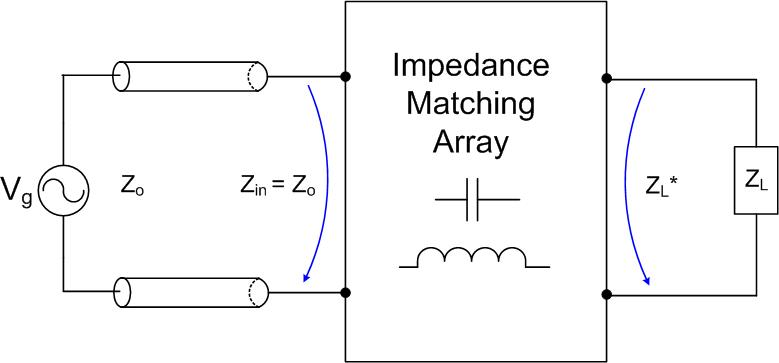
\includegraphics[scale=0.4]{../jpg/Impedancematching.jpg}
\end{center}
\caption{The result of impedance matching.}
\label{eq:impmatchgen1}
\end{figure}




\section{Simple impedance matching case}

The simplest impedance matching case is when the real part of the load impedance is already equal to the transmission line impedance. 

Let's say that the load impedance is $Z_L=R_L+j \omega L =50+j80 \Omega$ and needs to be matched to a $Z_0=50\Omega$ line. This impedance represents a resistor of $50\Omega$ connected in series with a $80 \Omega$-reactance inductor. The reactance of $80 \Omega$ is an inductor of inductance $12.73$nH at 1GHz.  

To make this impedance look like a $50 \Omega$ impedance, we have to add an element   with $Z_{add}=-j80 \Omega $ impedance, so that $Z_L+Z_{add}=50 \Omega$. Since this impedance is negative, we know that we have to add a capacitor. Because we are adding two impedances, we know that they must be in series. 

To look at this solution on the Smith Chart, we first normalize the impedance of the load $\bar{Z}_L=\frac{Z_L}{Z_0}=1+j1.6$, and then place it on the Smith Chart as shown in Figure \ref{fig:SimpleMatch} as a red dot. To get to the center of the Smitch Chart, we use only the resistance/conductance circles, because we know that on these circles only the reactance/susceptance of the impedance changes and we don't want to add resistors to change the real part of the impedance. We see that the circle we have to use is the $Z=1$ circle, because the load impedance  is on it.  To get to the center of the chart, where $Z=1$. To find the reactance we need to add, we subtract  the matched impedance Z and the load impedance $Z_{add}=Z- Z_L=-j1.6$. Another way to see that this is a capacitor is to notice that by adding this element, we are moving from the inductive (upper half) to capacitive part (lower part) of the Smith chart. 

\begin{figure}[htbp]
\begin{center}
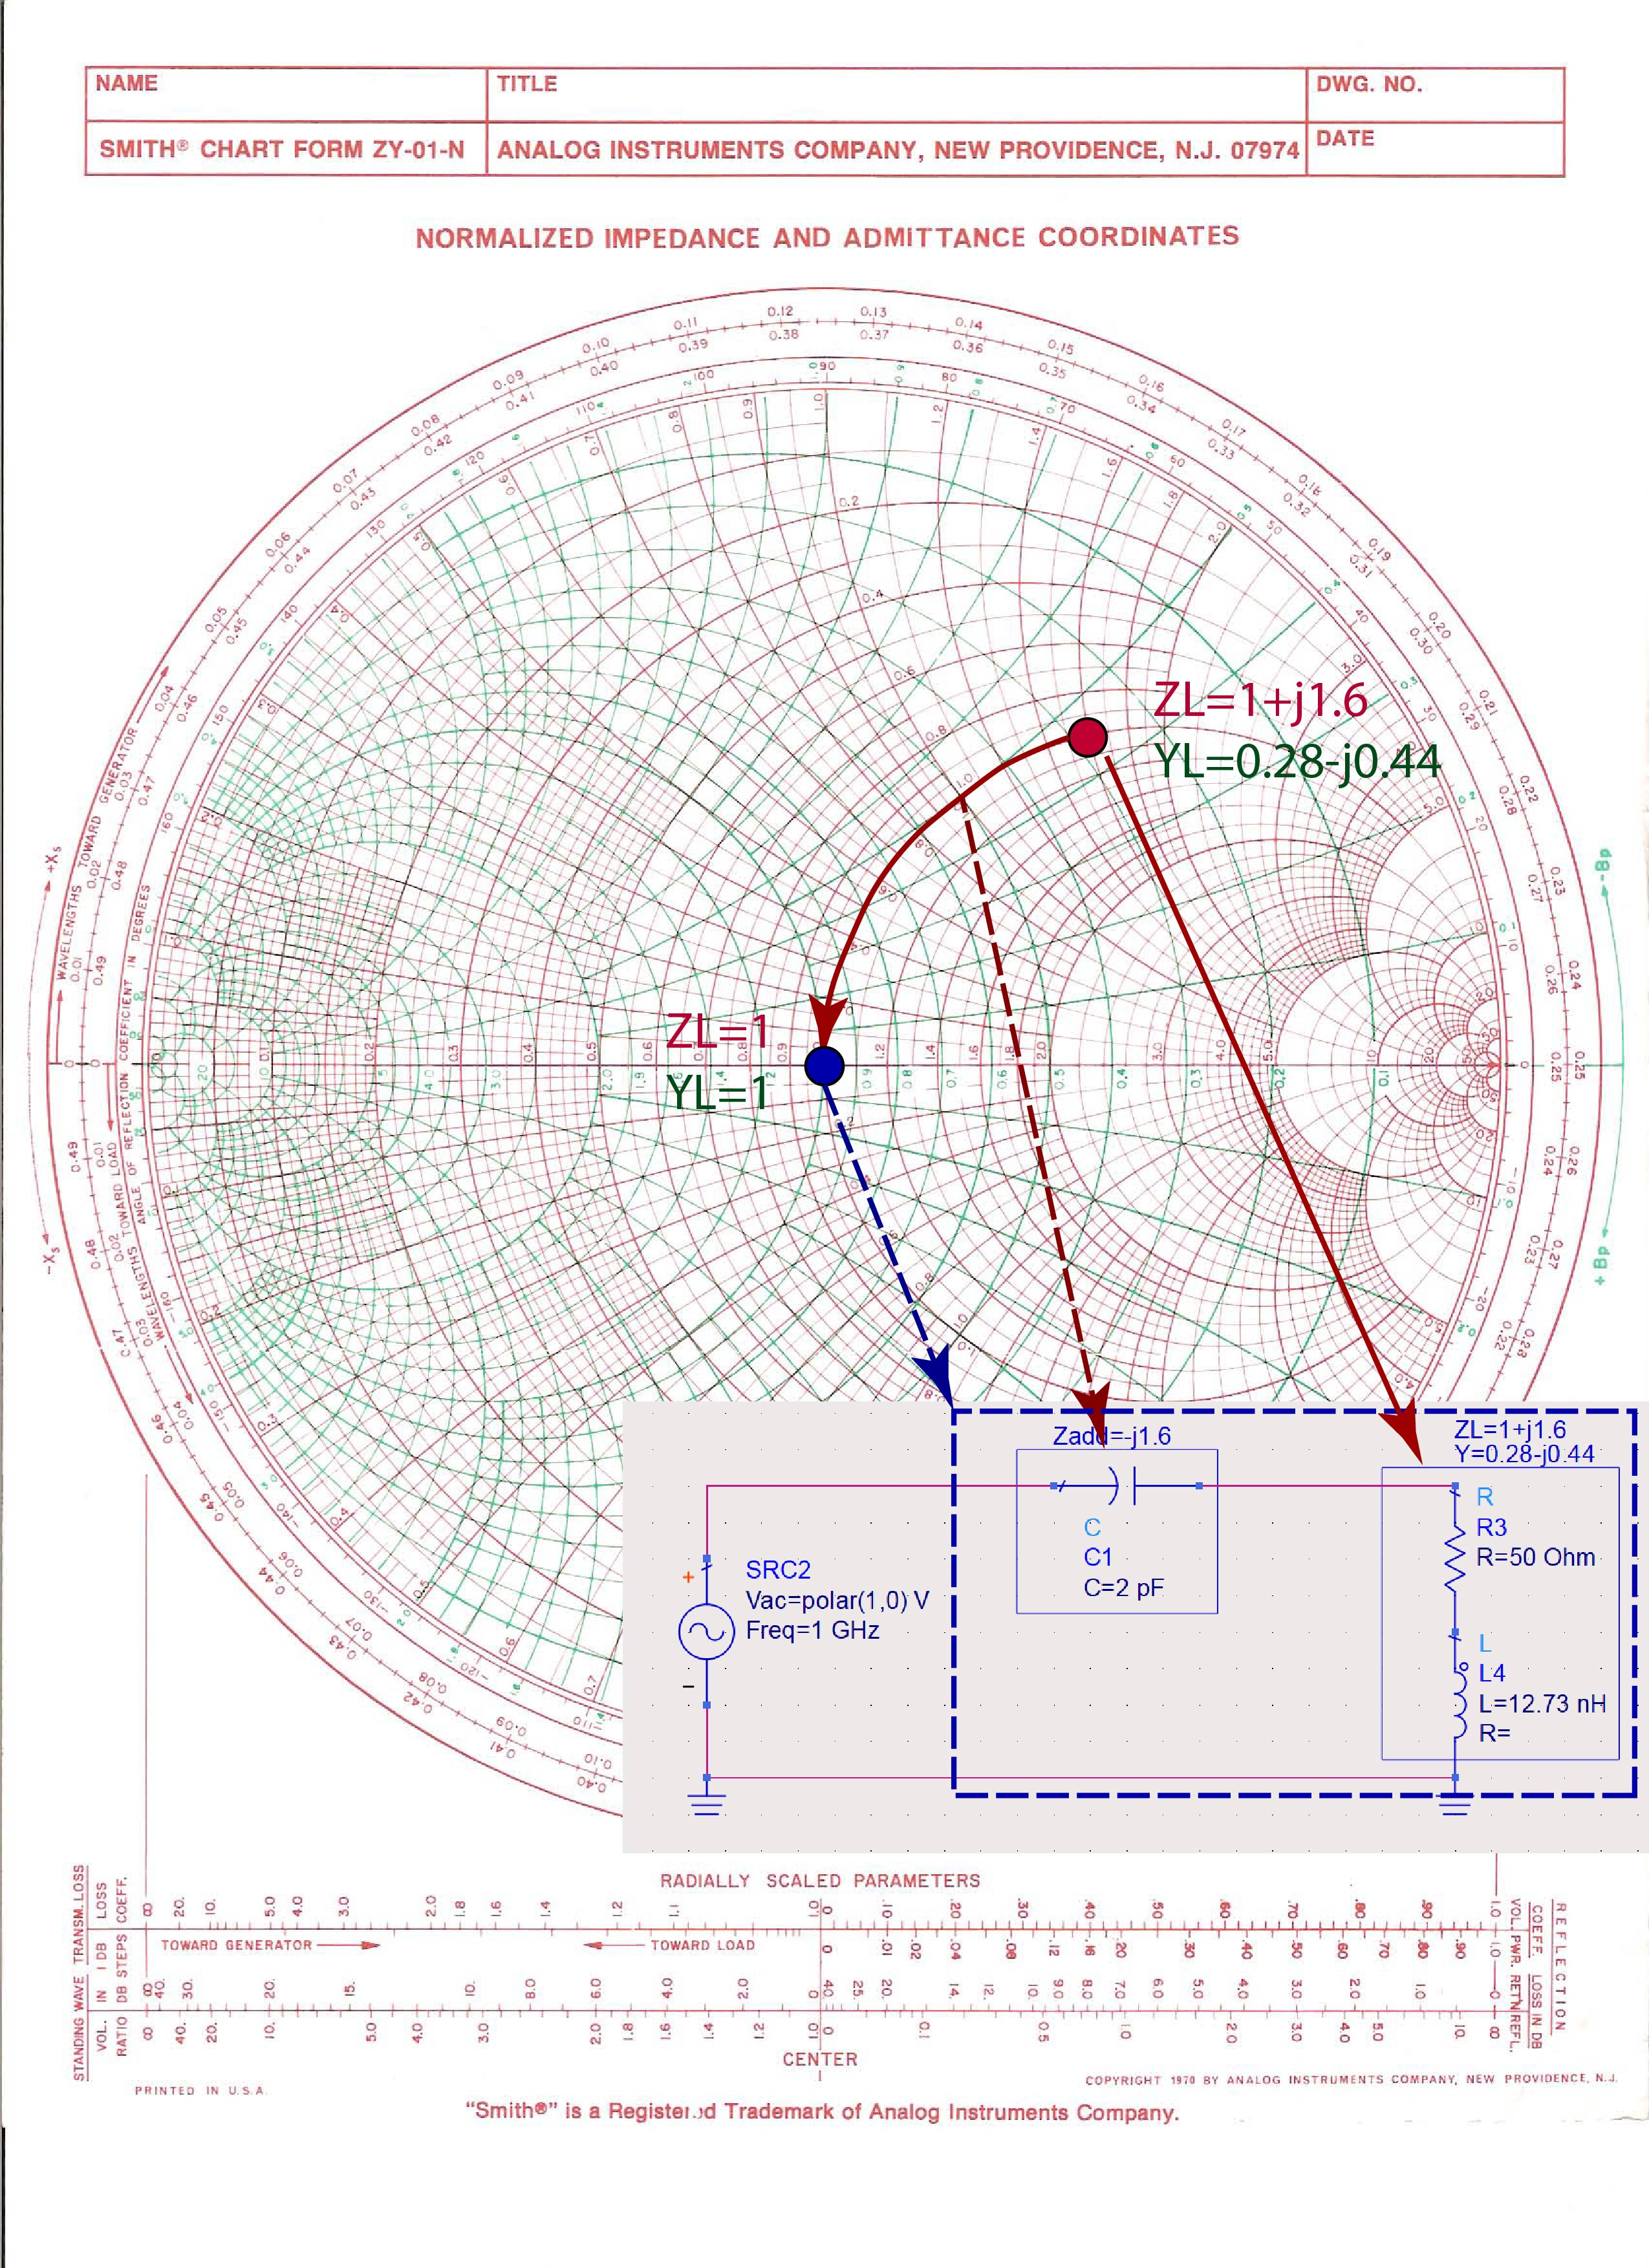
\includegraphics[scale=0.4]{../jpg/SimpleMatch-01.jpg}
\end{center}
\caption{The result of impedance matching.}
\label{fig:SimpleMatch}
\end{figure}

Finally, we have to find the capacitance of a $Z_{add}=-j1.6 50 \Omega$. The added impedance is multiplied by $50 \Omega$ to re-normalize the impedance. The impedance of any capacitor is $Z=\frac{1}{j \omega C}=-j \frac{1}{\omega C}$. To find the capacitance of this capacitor we set $-j \frac{1}{\omega C}=-j1.6 50$. From this equation, and keeping in mind that $\omega = 2 \pi f$, we calculate that the capacitance is $C \approx 2$pF.



\section{Design of mixed impedance matching circuits}

The real part of the load impedance of various circuits is rarely equal to the transmission-line impedance. For example, load impedance $Z_L=25+j 100 \Omega$ represents a series connection of a $25\Omega$ resistor and a $7.96$nH inductor at 1GHz.

Tp match $Z_L=25+j 100 \Omega$ impedance to the transmission-line impedance $Z_0=50 \Omega$ we first normalize the load impedance to transmission-line impedance.


\begin{equation}
\bar{Z}_L=\frac{Z_L}{Z_0}=0.5+j1
\end{equation}

This impedance is shown in Figure \ref{fig:PointSC}. 

\begin{figure}[htbp]
\begin{center}
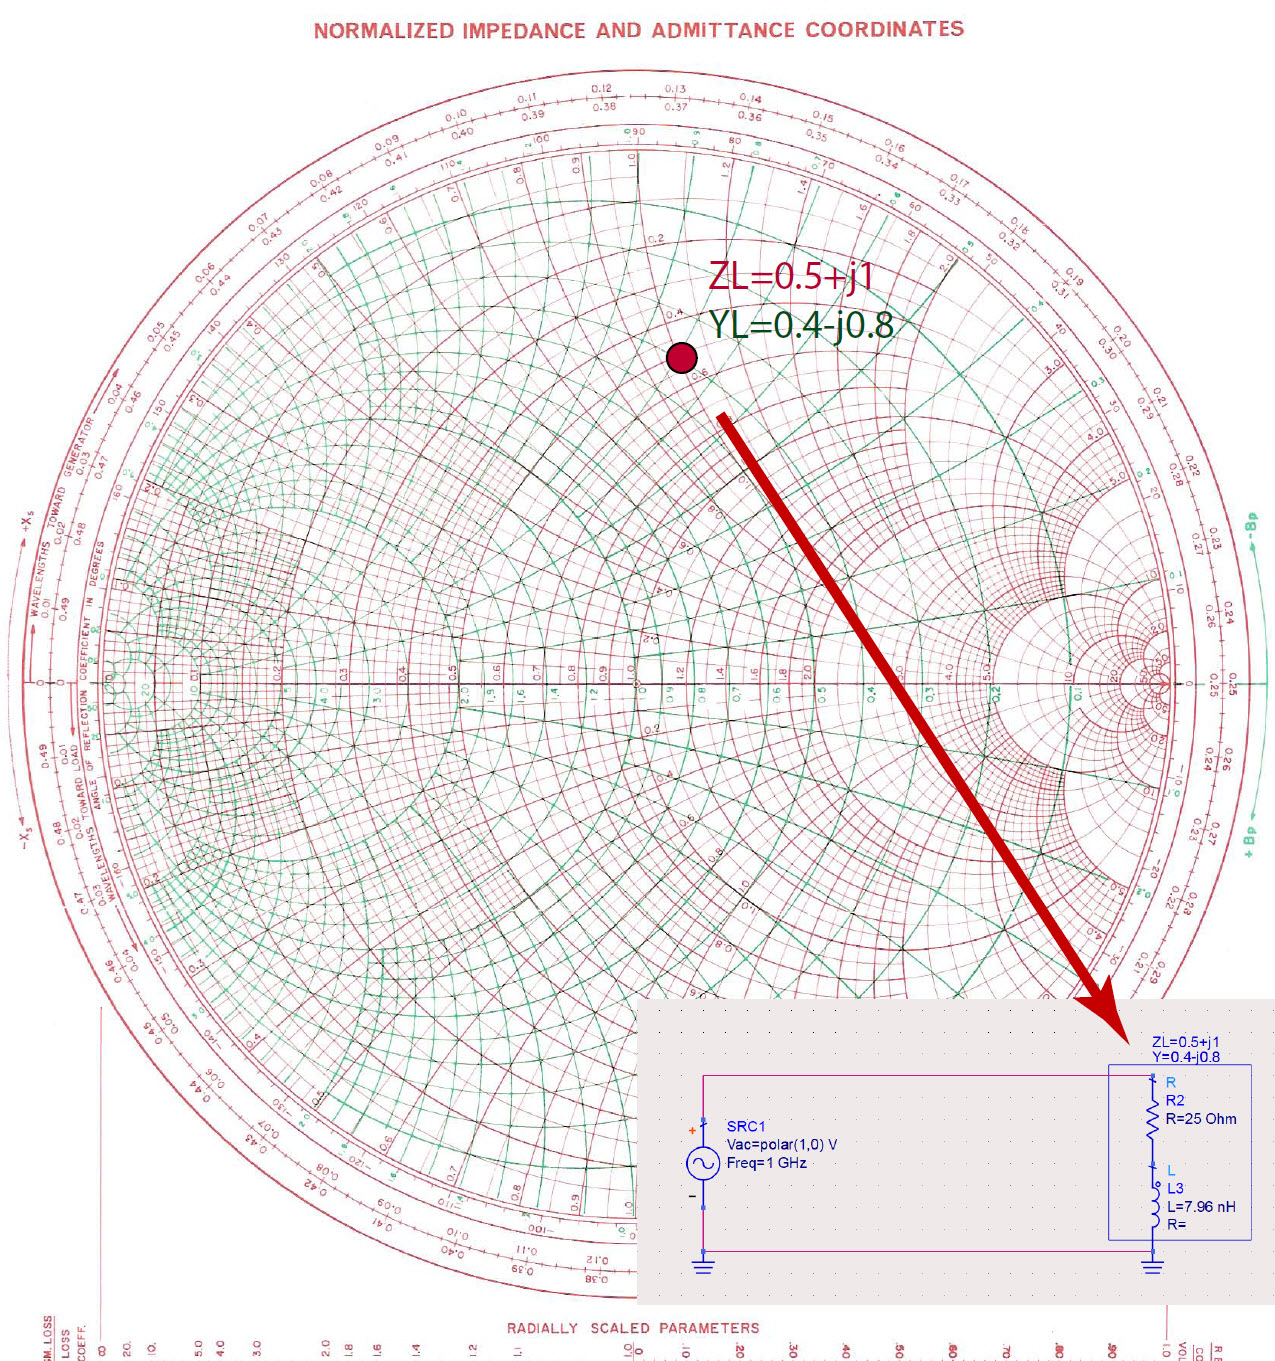
\includegraphics[scale=0.4]{../jpg/Match1.jpg}
\end{center}
\caption{Load impedance $Z_L=0.5+j1$ on Smith Chart.}
\label{fig:PointSC}
\end{figure}

Then, we identify an SWR circle that this impedance is on, as shown in Figure \ref{fig:SWRfor25Ohm}. The point where the SWR circle intersect the green circle where the real part of the input admittance is equal to one $Y_1=1$ will give us the length of the line that we have to add to the load impedance. 

To find the length of the line, we identify the position of the load impedance $Z_L=0.5+j1$ and the input impedance $Z_1=0.3-j0.45$ at the {\it Wavelengths Towards Generator} (WTG) scale. Load impedance is at $0.135 \lambda$, and the input impedance is at $0.425 \lambda$. The difference between these two positions gives us the length of the line $0.29 \lambda$. In electrical degrees, this lenght is approximately $105^0$. The input admittance to the line is now $Y_L=1+1.6$.

\begin{figure}[htbp]
\begin{center}
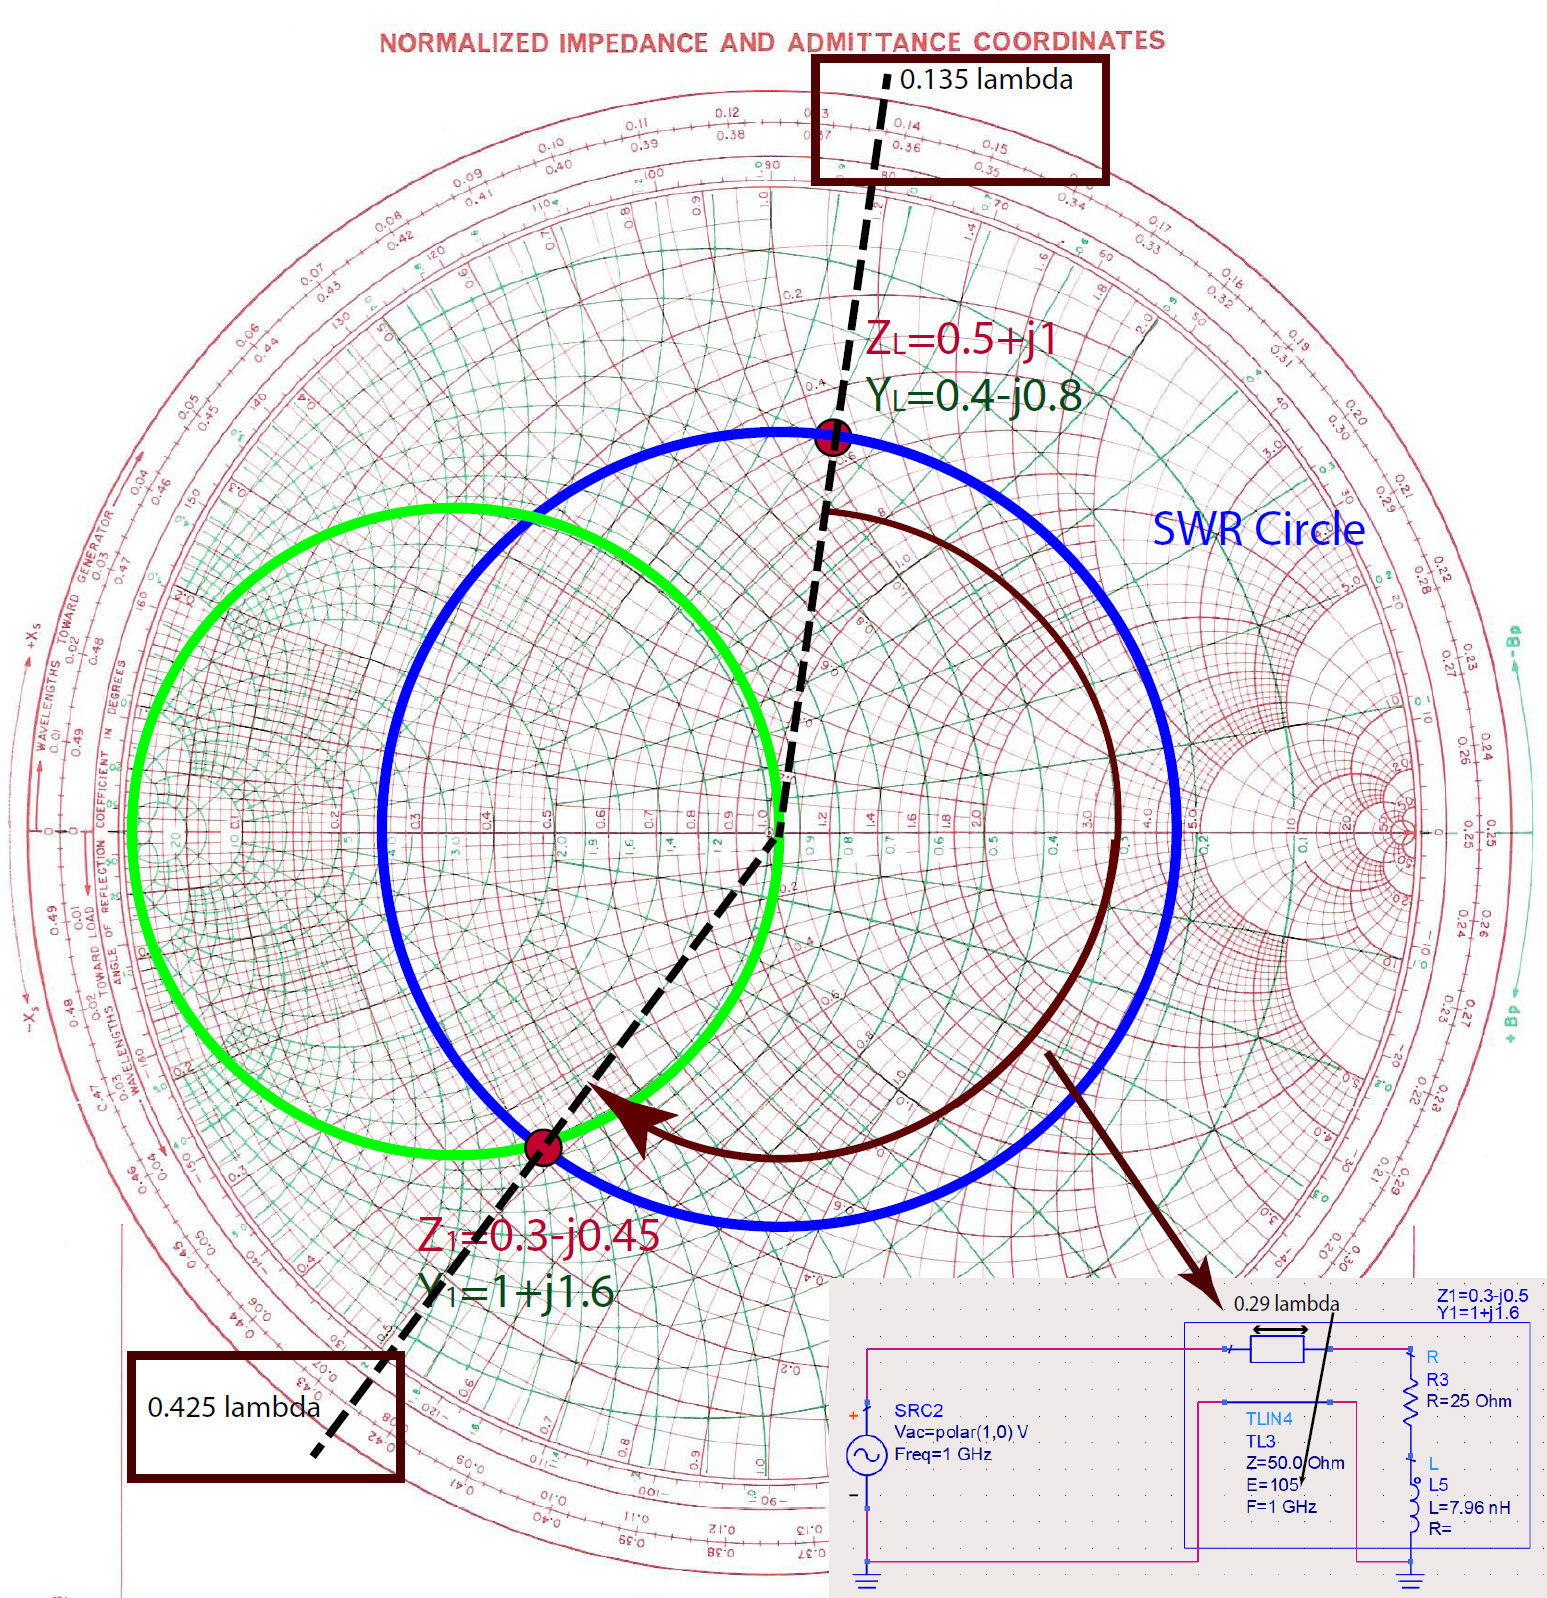
\includegraphics[scale=0.4]{../jpg/Match2.jpg}
\end{center}
\caption{SWR circle for impedance $Z_L=0.5+j1$.  }
\label{fig:SWRfor25Ohm}
\end{figure}


The final step is to add a susceptance that will remove the imaginary part of the input admittance $Y_1=1+j 1.6$. We see that to get the final admittance of $Y_M=1$, numerically, we have to add an admittance of $Y_{add}=-j1.6$. This represents an anductance. Since we are adding the two admittances $Y_1+Y_{add}$, they have to be in parallel (as we know that when elements are in parallel, we add their admittances).


\begin{figure}[htbp]
\begin{center}
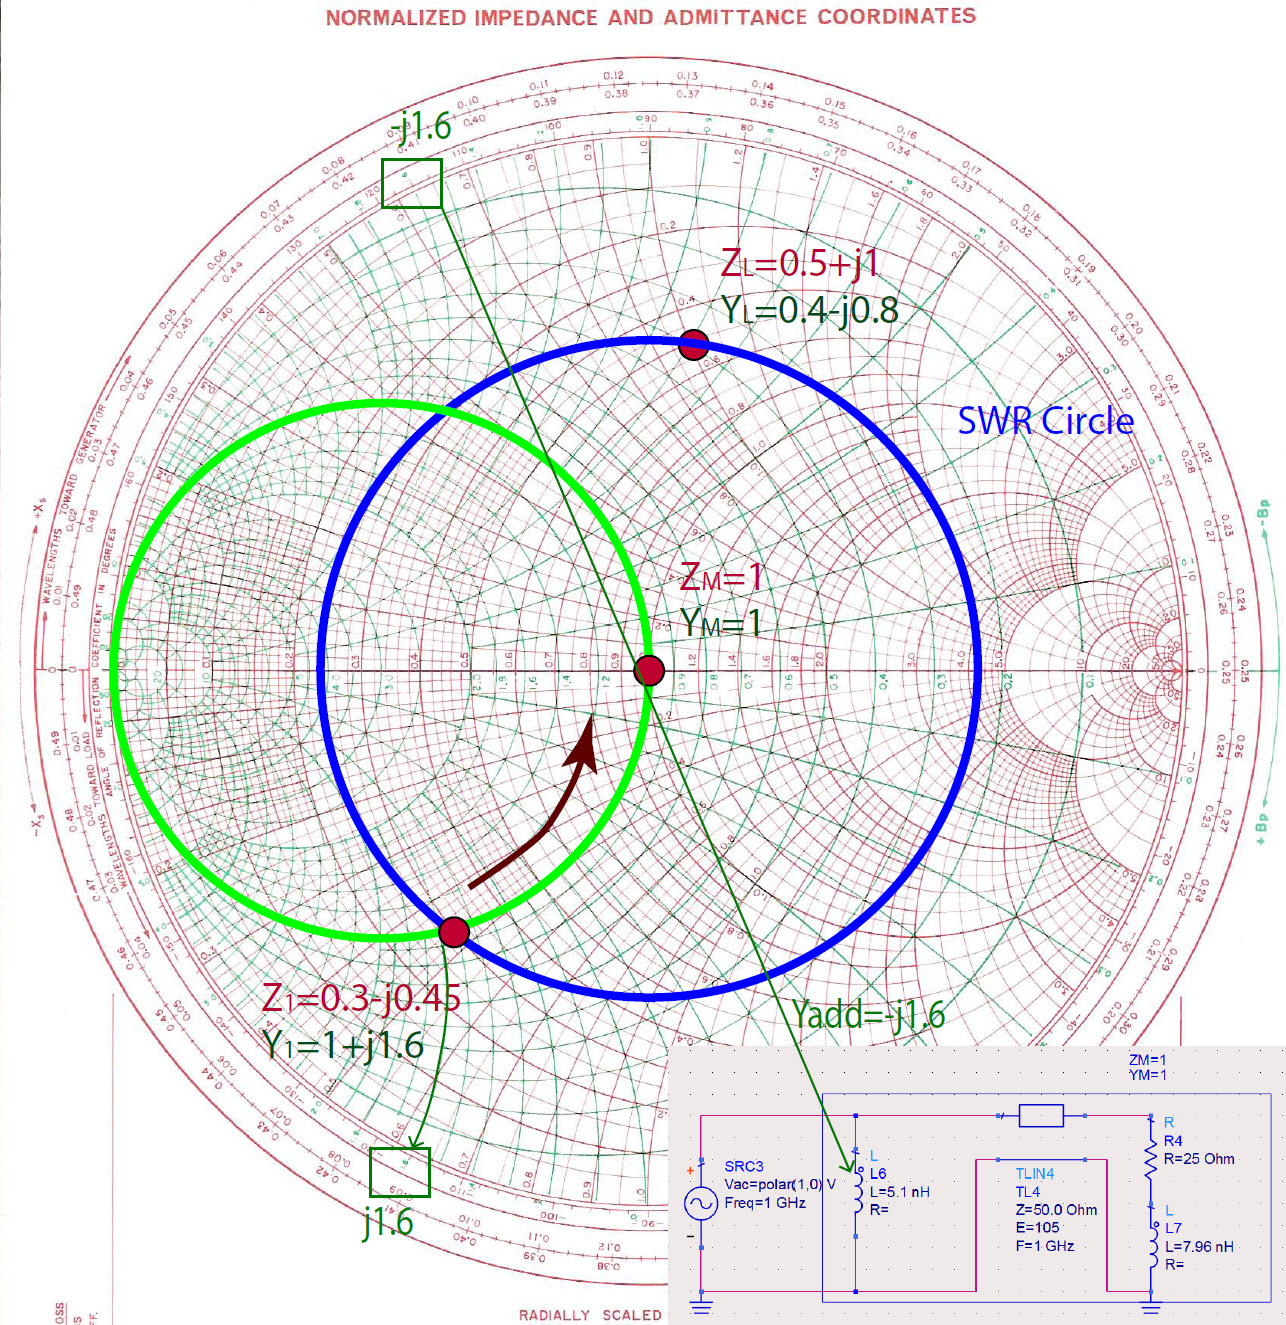
\includegraphics[scale=0.4]{../jpg/MatchMixed1.jpg}
\end{center}
\caption{The result of impedance matching.}
\label{impmatchgen}
\end{figure}
\newpage

Graphically, there are several different mixed or tranmission-line impedance matching circuits that we can make for a specific impedance. For example,for impedance $Z_L=25+j50 \Omega$, there are four different  circuits that we can make, as shown in Figure \ref{fig:MixedVariety}. In this paragraph we used the green path on the Smith Chart, with intermediate admittance $Y_2$. 


\begin{figure}[htbp]
\begin{center}
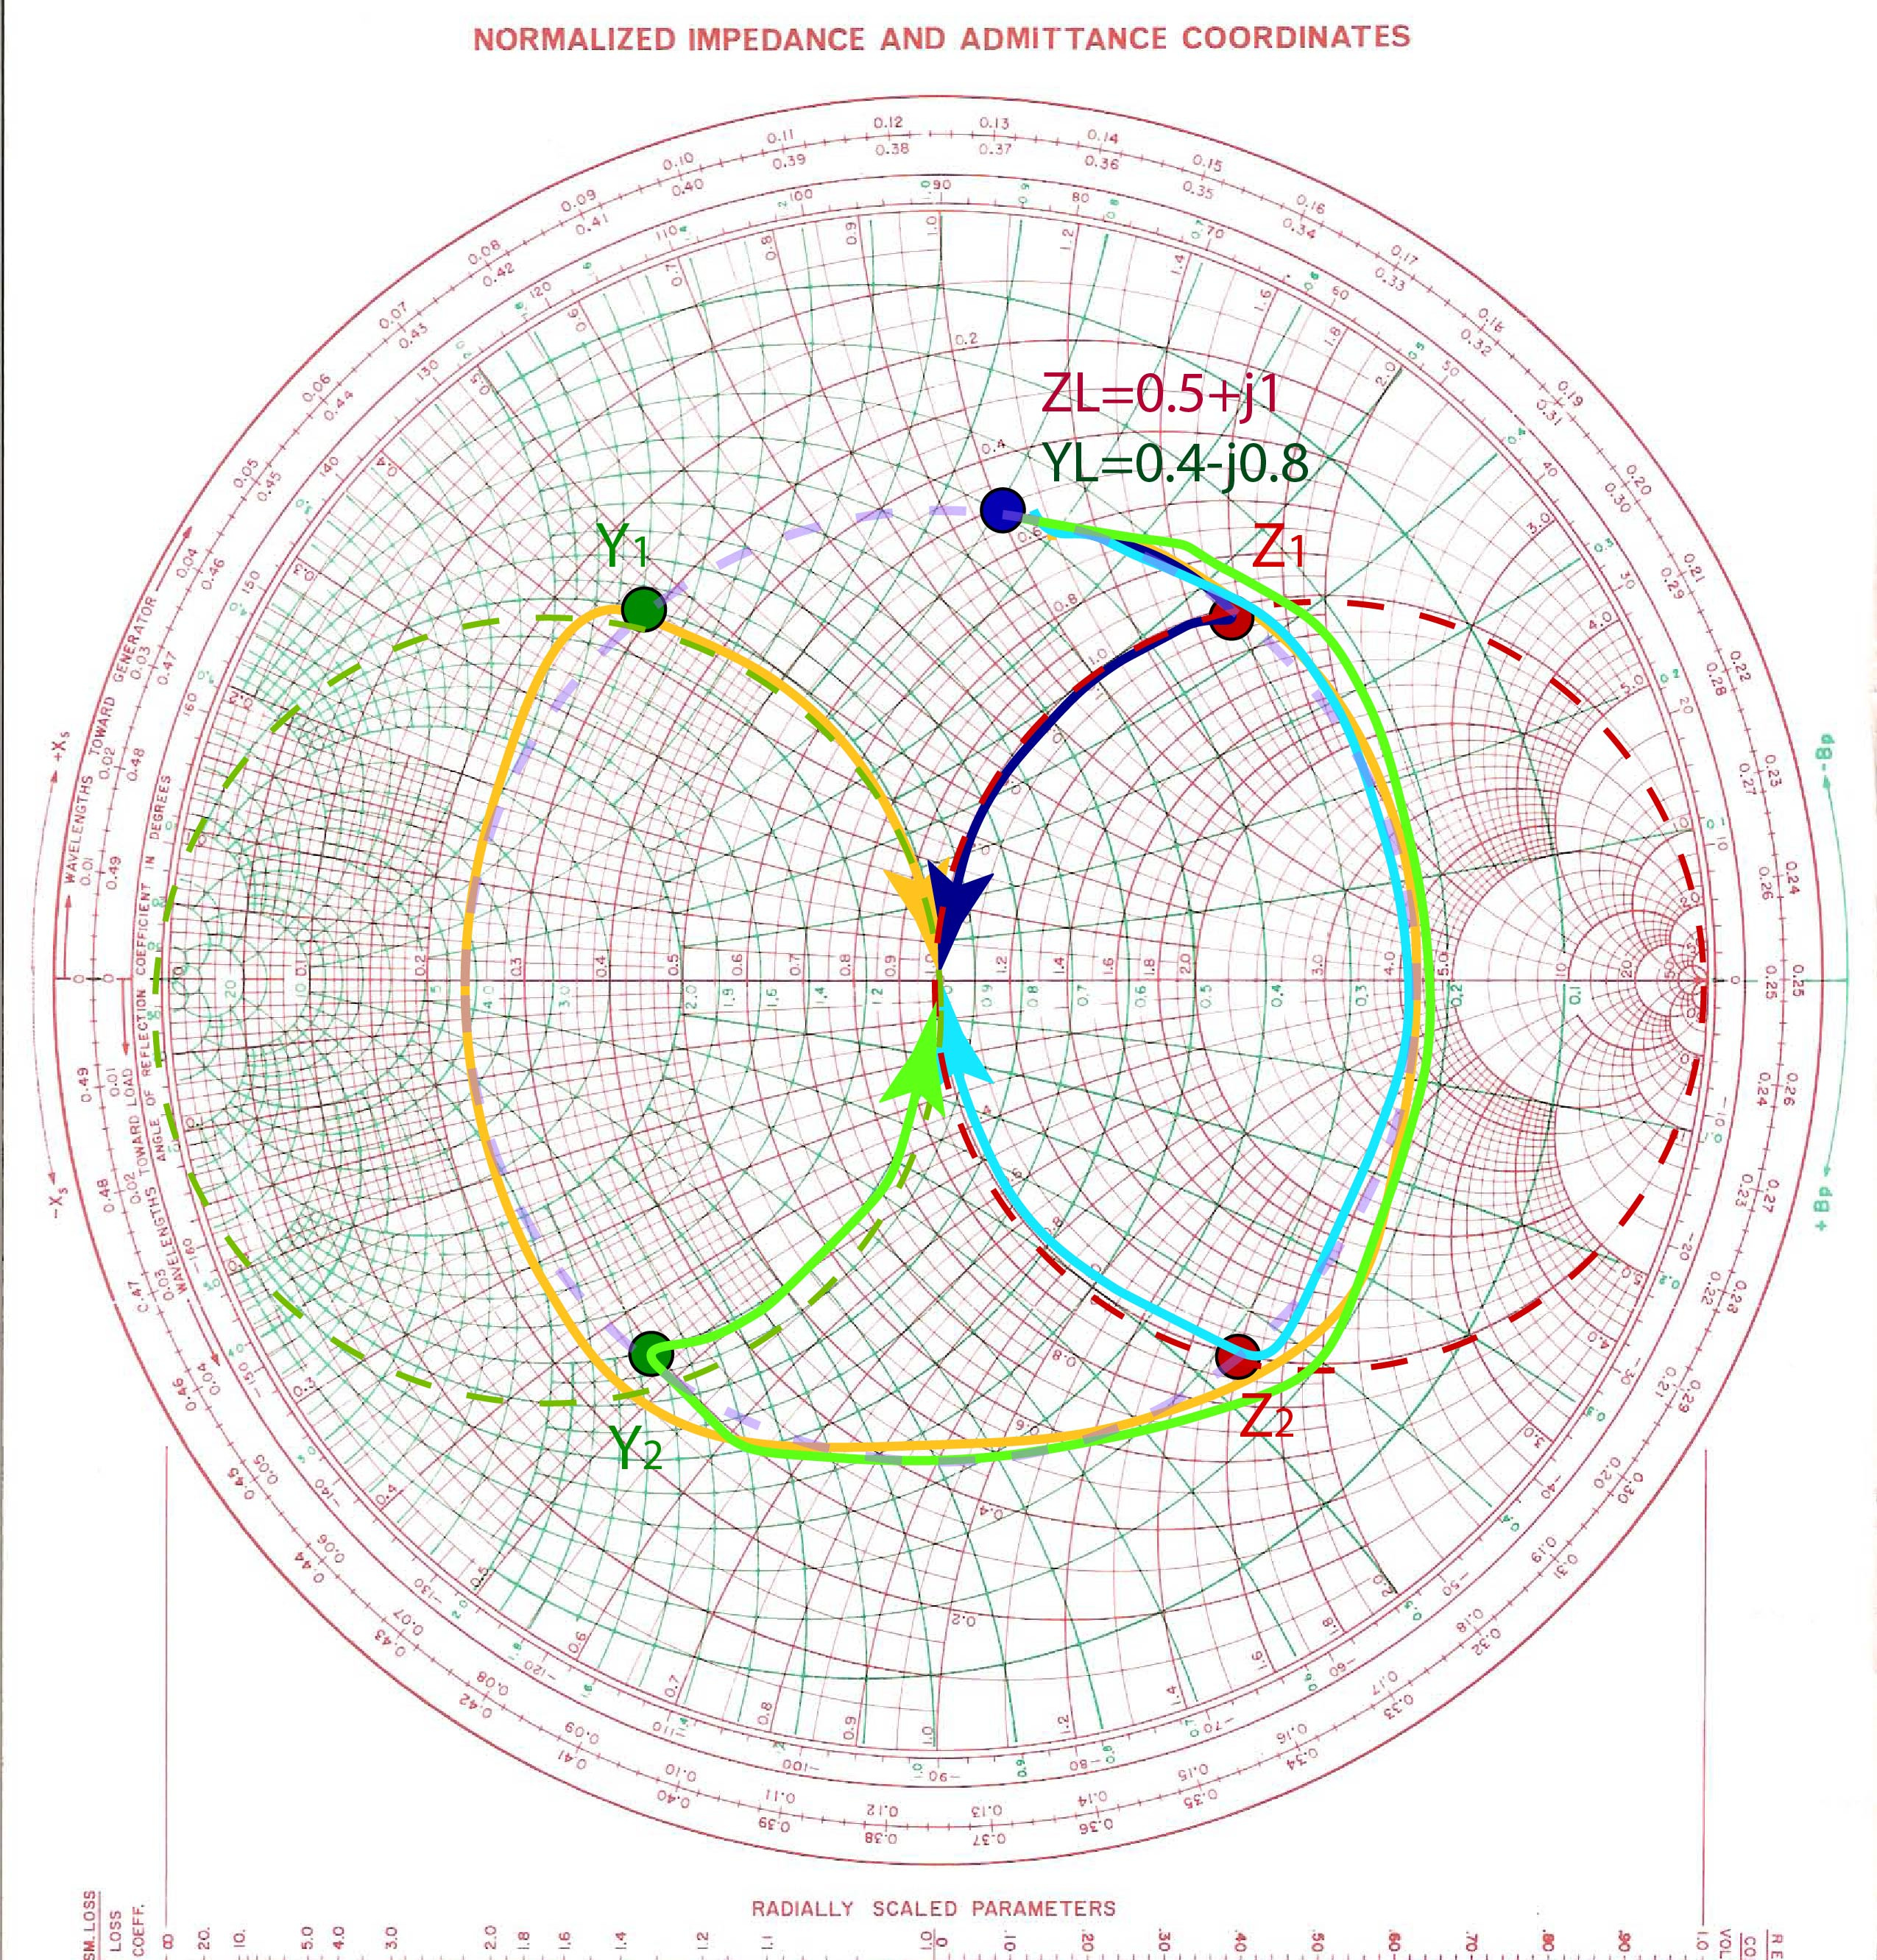
\includegraphics[scale=0.4]{../jpg/MixedVariety-01.jpg}
\end{center}
\caption{A variety of possible impedance matching circuits for impedance $Z_L=25+j50 \Omega$.}
\label{fig:MixedVariety}
\end{figure}




\section{Design of a transmission-line impedance matching circuits}

Transmission-line impedance matching circuits are used at higher frequencies where the lumped elements become very small, and impractical to use. 

To design fully transmission-line matching circuits, we have to first learn how to replace the lumped element in the matching circuit from the last step in the previous section with a transmission line. 


\subsection{Replacing lumped-elements with equivalent transmission-line stubs}

To make fully transmission line impedance matching circuits, we can replace capacitors and inductors  with ``stubs", which are shorted or open transmission lines. 

Input impedance of shorted or open transmission lines  can be made purely inductive or capacive, as shown in Figures \ref{fig:OpenStubLambdaOver8}-\ref{fig:ShortedStubLambdaOver8}. SWR circle of an open or shorted stub is the outer perimeter of the Smith Chart. The length of the transmission line will determine the input impedance of the stub. The input impedance is always purely reactive. 

For example, in Figure \ref{fig:OpenStubLambdaOver8}, the length of the line is  $\frac{\lambda}{8}$. The ``load" connected to the output of this line is an open circuit $Z_L=\infty$. On the Smith Chart we start from the load impedance, and add a $0.125 \lambda$ line, following the WTG scale. The input impedance is purely capacitive $Z_{in}=-j$. 

\begin{figure}[htbp]
\begin{center}
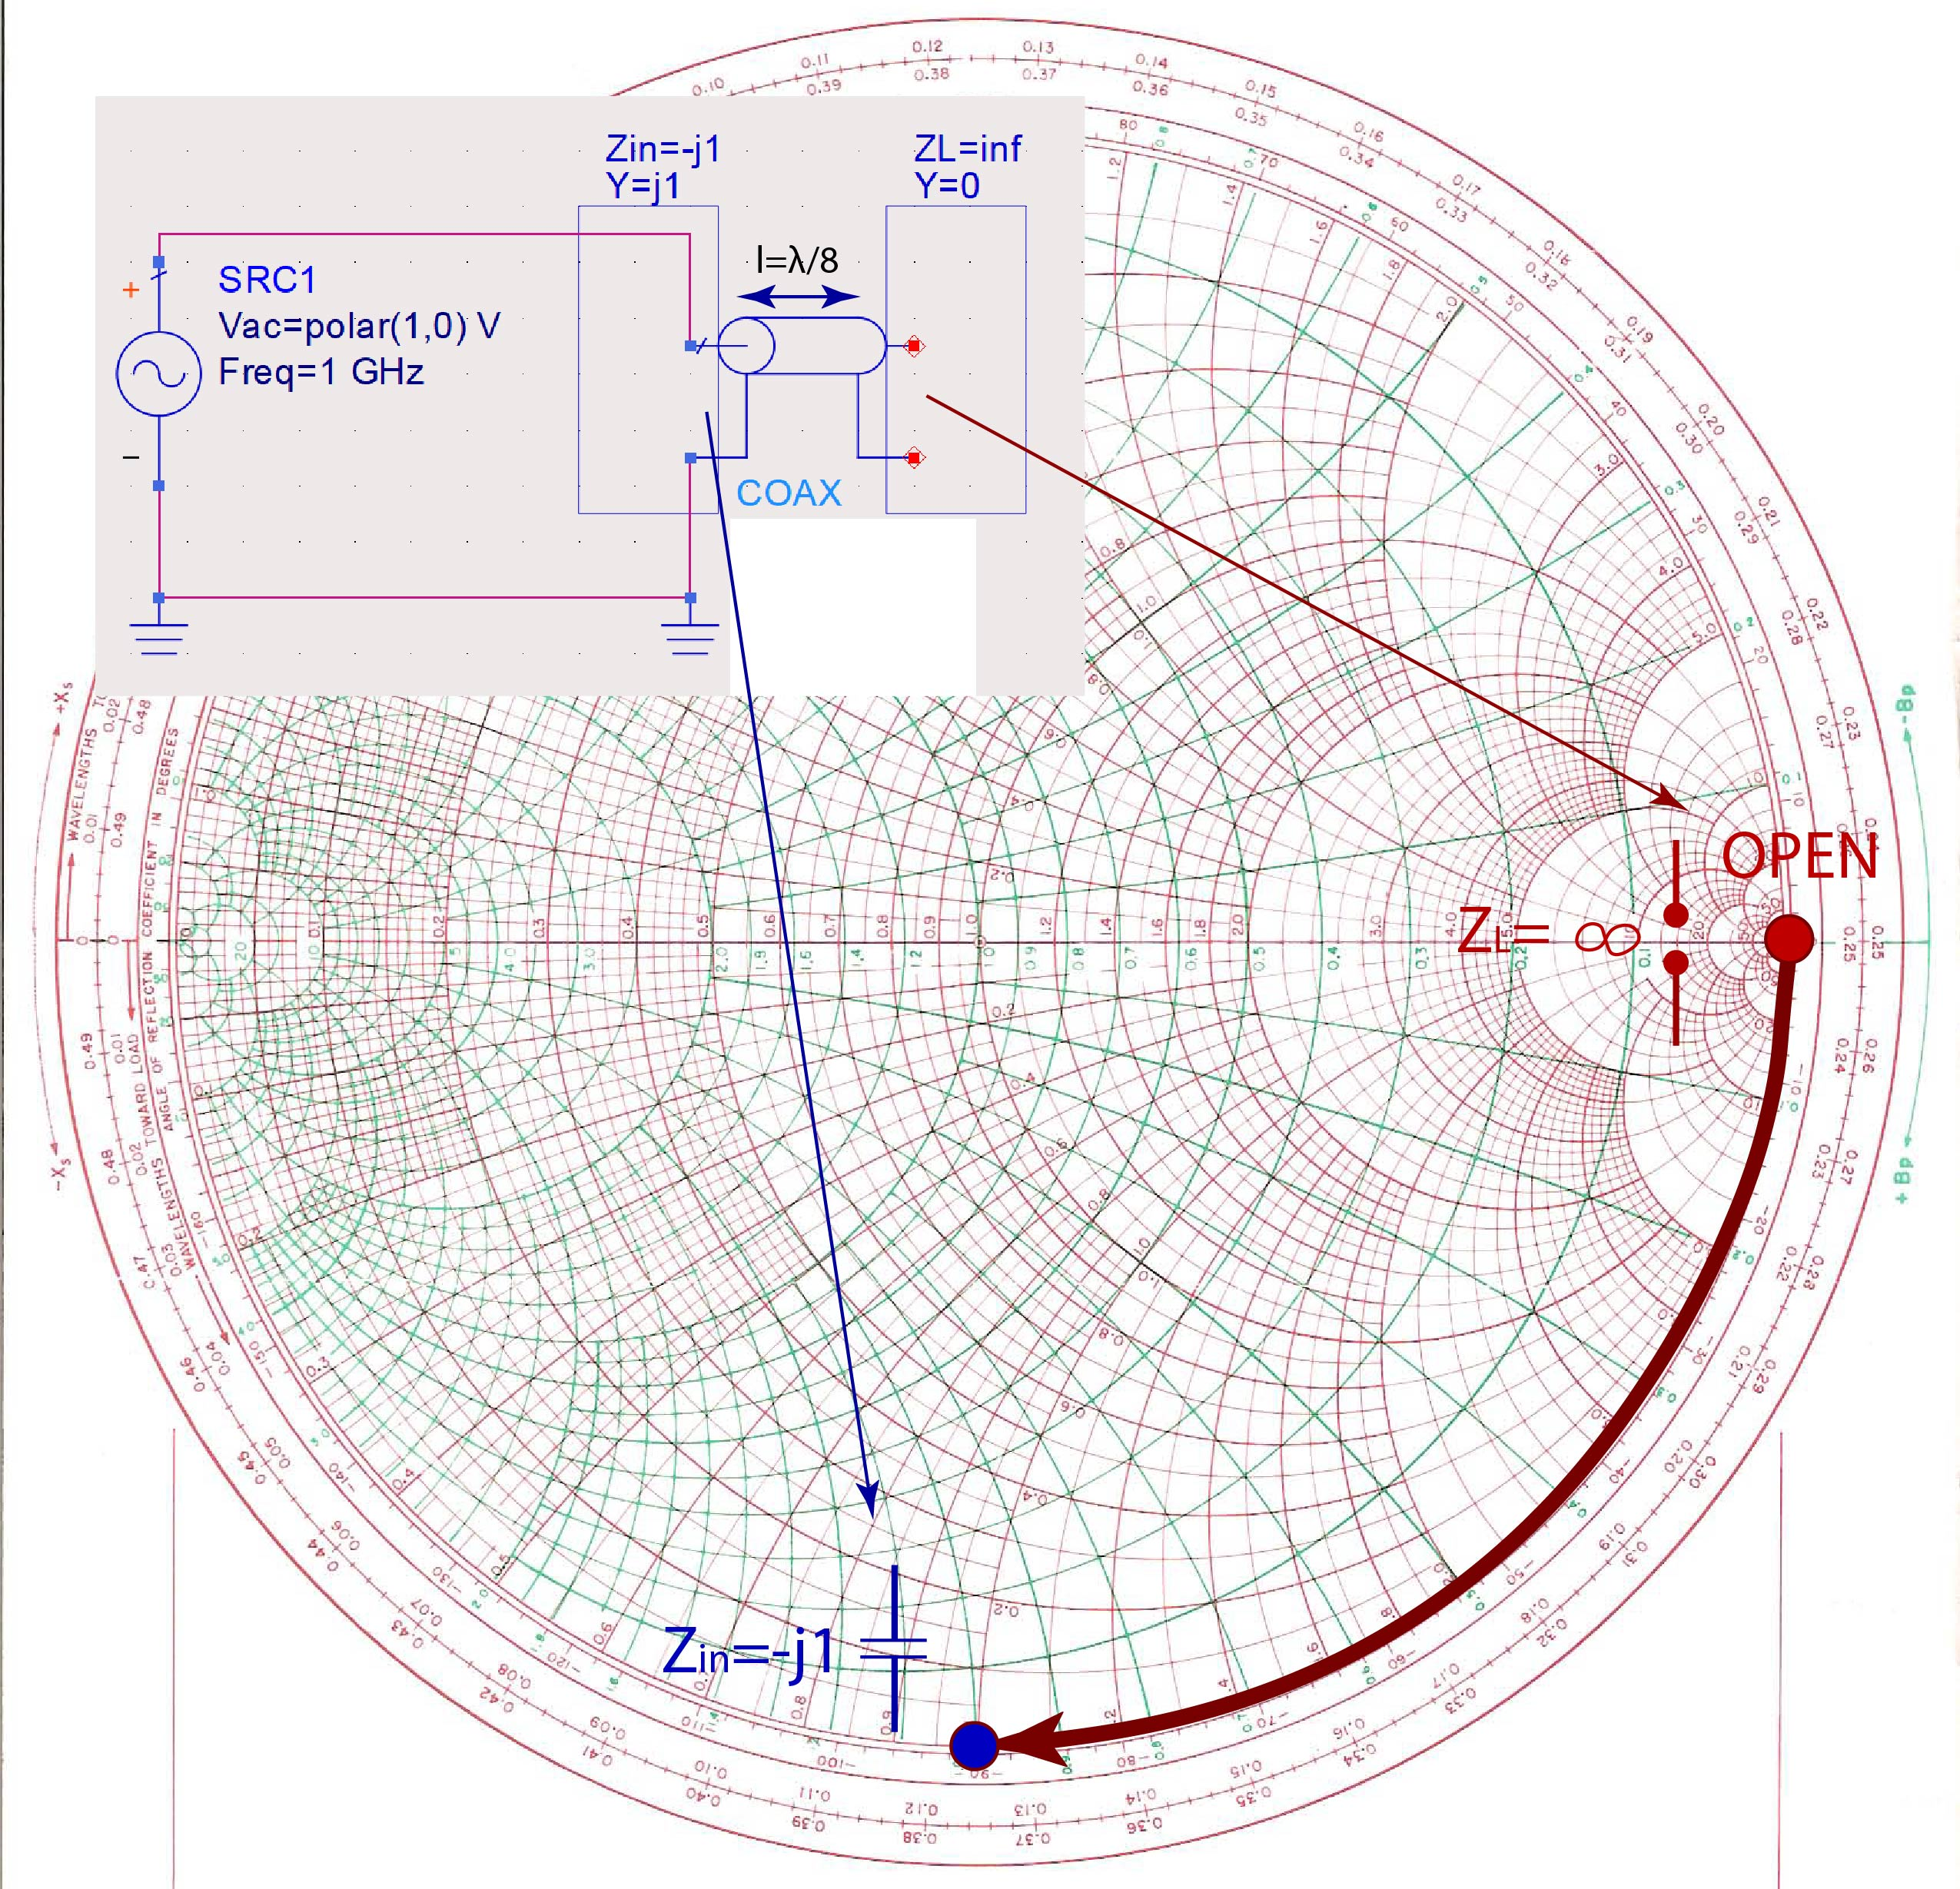
\includegraphics[scale=0.4]{../jpg/openstub-01.jpg}
\end{center}
\caption{Input impedance $Z_{in}=-j$ of a $\frac{\lambda}{8}$ open transmission line.}
\label{fig:OpenStubLambdaOver8}
\end{figure}

The input impedance  is equal to a capacitor's impedance $Z_{in}=-j$ at a single frequency, where the electrical length of the line is $0.125 \lambda$. At other frequencies, the electrical length of the line is different, and therefore the input impedance is lower or higher than $Z_{in}=-j$.



Another example is shown in Figure \ref{fig:OpenStub3LambdaOver8}, where the length of the line is  $\frac{3 \lambda}{8}$. The load connected to this line is again an open circuit $Z_L=\infty$. On the Smith Chart we start from the load impedance, and add a $0.375 \lambda$ line, following the WTG scale. The input impedance is purely inductive $Z_{in}=j$.

\begin{figure}[htbp]
\begin{center}
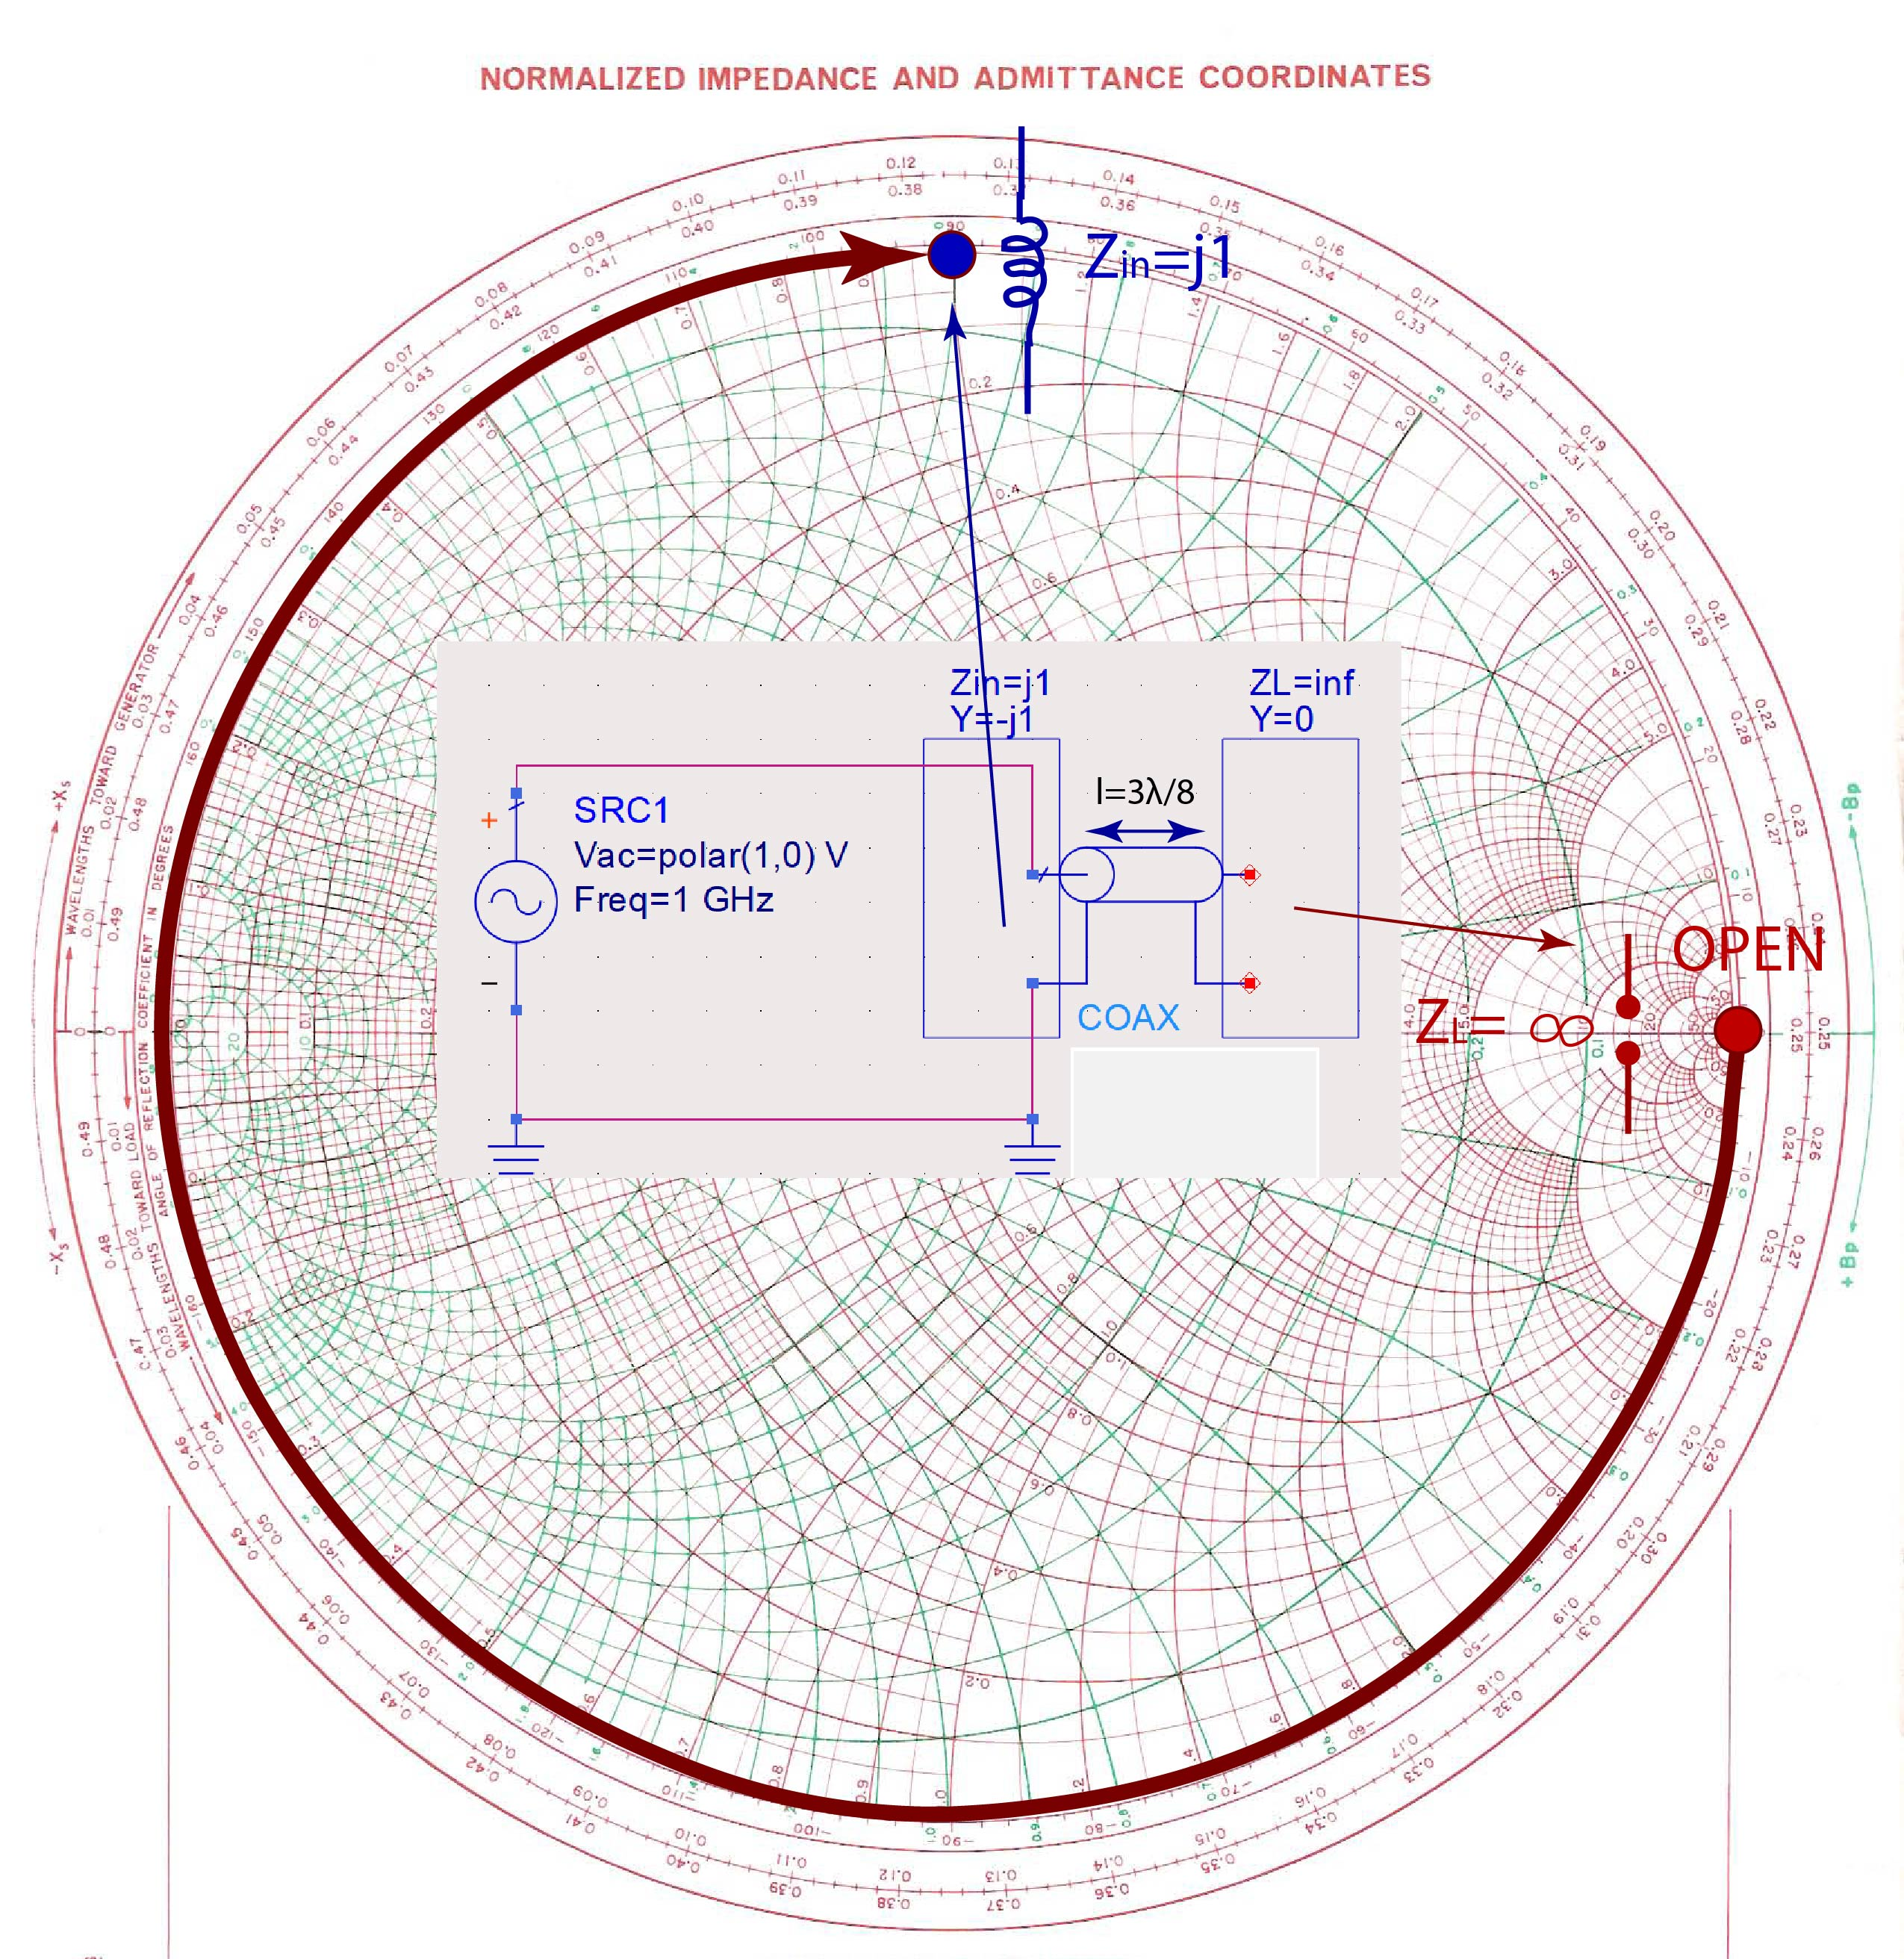
\includegraphics[scale=0.4]{../jpg/openstub2-01.jpg}
\end{center}
\caption{Input impedance $Z_{in}=j$  of a $\frac{3 \lambda}{8}$ open transmission line.}
\label{fig:OpenStub3LambdaOver8}
\end{figure}


The last example is shown in Figure \ref{fig:ShortedStubLambdaOver8}, where the length of the line is  $\frac{3 \lambda}{8}$. The load connected to this line is now a short circuit $Z_L=0 \Omega$. On the Smith Chart we start from the load impedance, and add a $0.375 \lambda$ line, following the WTG scale. The input impedance is purely inductive $Z_{in}=j$.



\begin{figure}[htbp]
\begin{center}
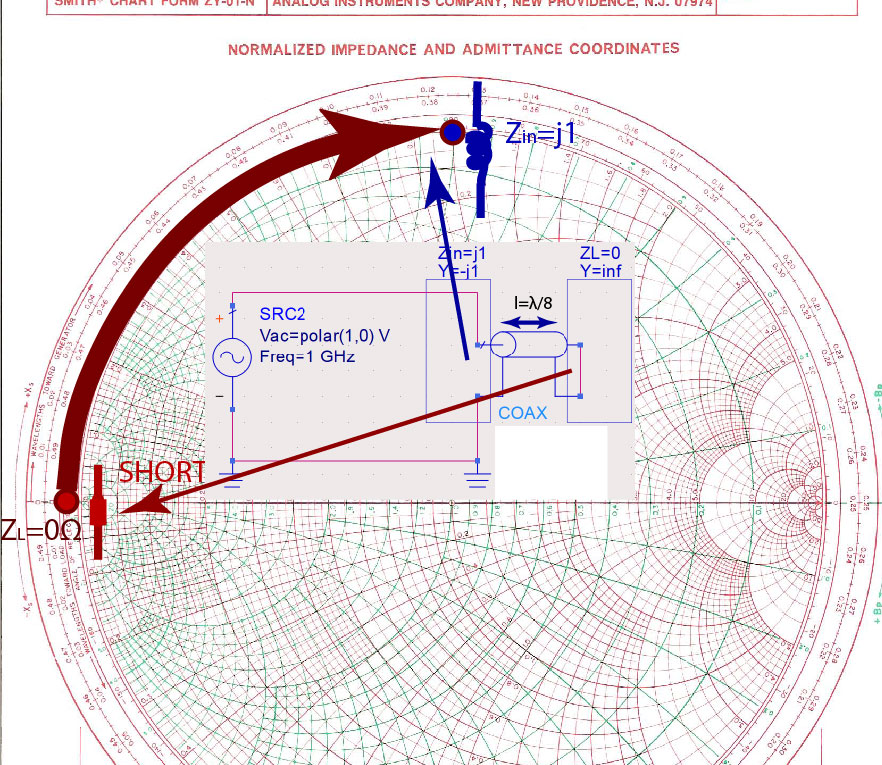
\includegraphics[scale=0.4]{../jpg/shortedstub-01.jpg}
\end{center}
\caption{Input impedance $Z_{in}=j$ of a $\frac{\lambda}{8}$ shorted transmission line.}
\label{fig:ShortedStubLambdaOver8}
\end{figure}
\newpage

\subsection{Fully transmission-line matching circuits.}

The first few steps in the fully transmission-line matching circuit are the same as in the mixed-impedance matching. We find the point on the Smitch Chart that represents the normalized impedance of the load $Z_L=0.5+j1$, as in Figure \ref{fig:NormImponSC}. 

\begin{figure}[htbp]
\begin{center}
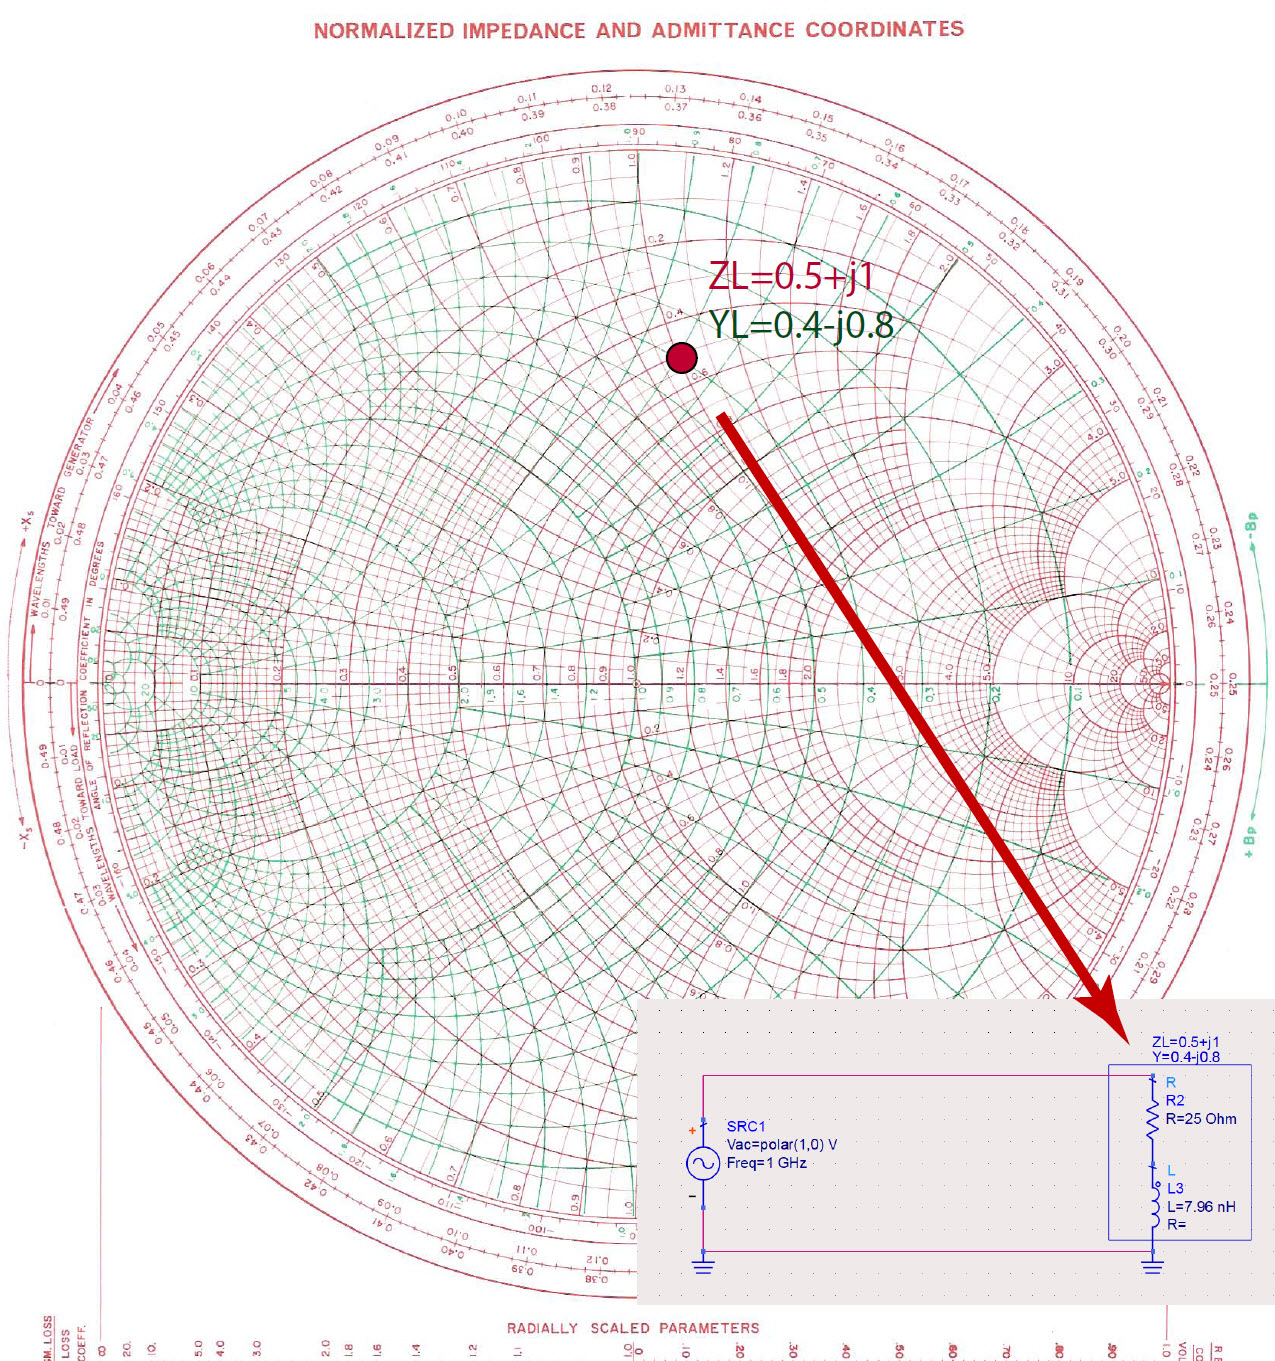
\includegraphics[scale=0.4]{../jpg/Match1.jpg}
\end{center}
\caption{Position of normalized impedance $Z_L=0.5+j1$ on Smith Chart.}
\label{fig:NormImponSC}
\end{figure}

A section of transmission line has to be added to impedance $Z_L=0.5+j1$ to transform the load impedance to input admittance $Y_{in}=1+1.6$, as shown in Figure \ref{fig:AddingSectionOfLine}. The length of the line is calculated by reading the position of the load impedance and input impedance on the WTG circle. Load impedance is at $0.135 \lambda$, and the input impedance is at $0.425 \lambda$. The difference between these two positions gives us the length of the line $0.29 \lambda$. In electrical degrees, this length is approximately $105^0$. The input admittance to the line is now $Y_L=1+1.6$. 


\begin{figure}[htbp]
\begin{center}
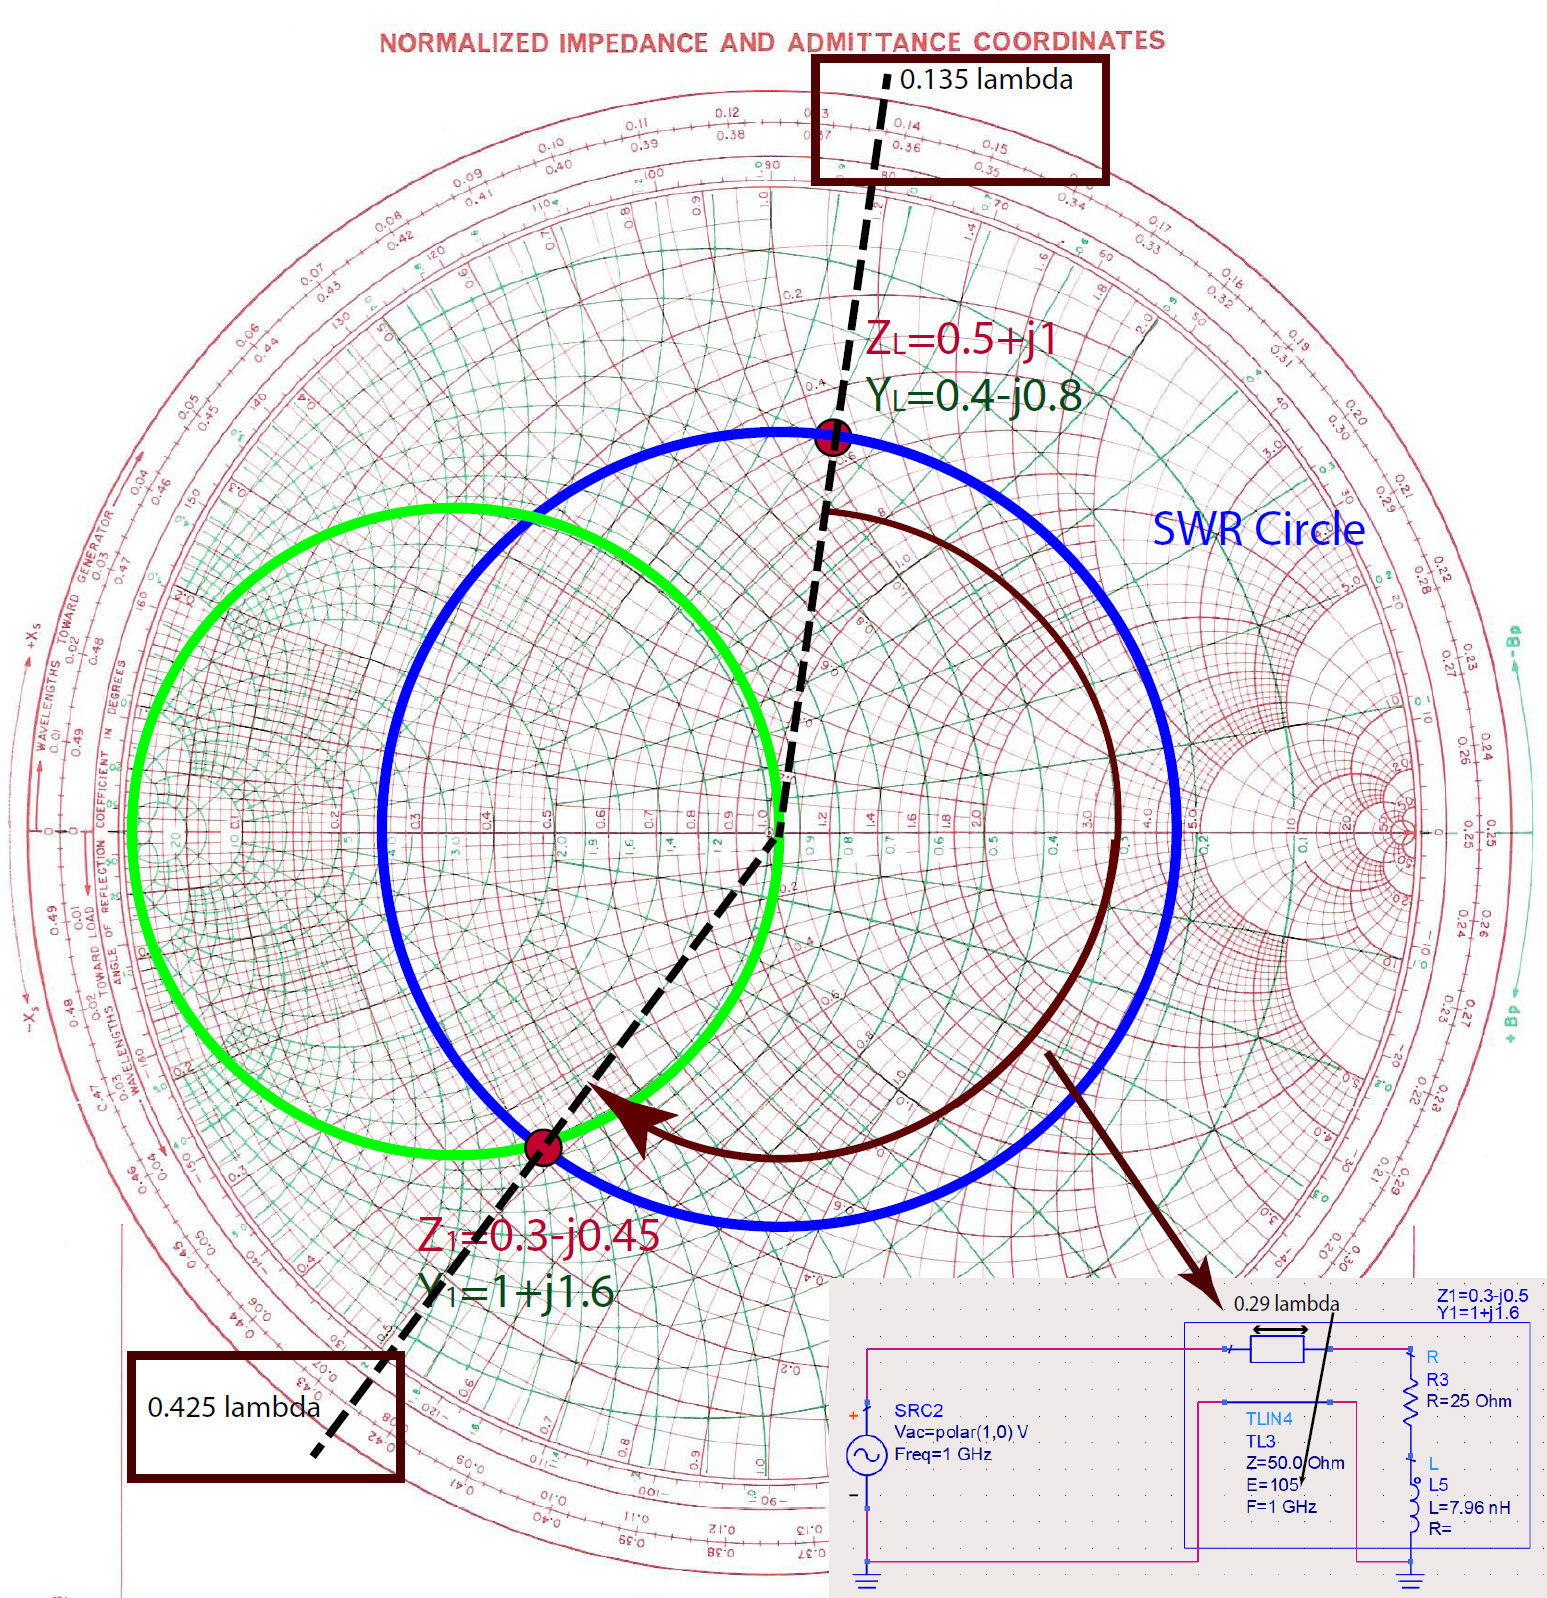
\includegraphics[scale=0.4]{../jpg/Match2.jpg}
\end{center}
\caption{The result of impedance matching.}
\label{fig:AddingSectionOfLine}
\end{figure}

The last step is to determine the shunt reactance that will remove the reactive part of the admittance $Y_L=1+1.6$, and make the total input impedance and admittance $Z_M=Y_M=1$. By inspection, we have to add $Y_{add}=-j1.6$. A lumped element in parallel (because we are adding two admittances), as in the previous mixed-matching problem, is an inductor (because admittance of an inductor is negative)  $Y_{add}=\frac{1}{j \omega L}=-j1.6$. However, we want to make a fully transmission line impedance matching circuit. Therefore, we have to replace the inductor with an equivalent transmission line, a stub. 

We can pick whether the stub is open or shorted. Usually, we want to pick the shortest possible stub, because the smaller the stub, the smaller the circuit will be. In some other cases, it is easier to leave the transmission line open, because making a short circuit requires drilling the PC Board and making a via-hole to connect the line to the ground. In this case, we picked an open stub to replace the lumped element, as shown in Figure \ref{fig:TransLineImpM}.

To find the stub that will have the same input admittance as an inductor $Y_{add}=-j1.6$, we first identify the position of admittance $-j1.6$ on the Smith Chart. This is the input impedance of the stub. We picked an open circuit for the load of the stub. To find the lenght of the stub, we start on the position of WTG scale from the load $Z_L=\infty$, WTG=$0.25 \lambda$, going in the WTG direction, we pass the short circuit position WTG=$0$, and then another WTG=$0.09 \lambda$ to reach the input admittance of $-j1.6$. The lenght of the stub is $0.25 \lambda+0.09 \lambda=0.34 \lambda$. In electrical degrees, this length is $\Theta=\beta l =2 \pi 0.34 \approx 123^0$.




\begin{figure}[htbp]
\begin{center}
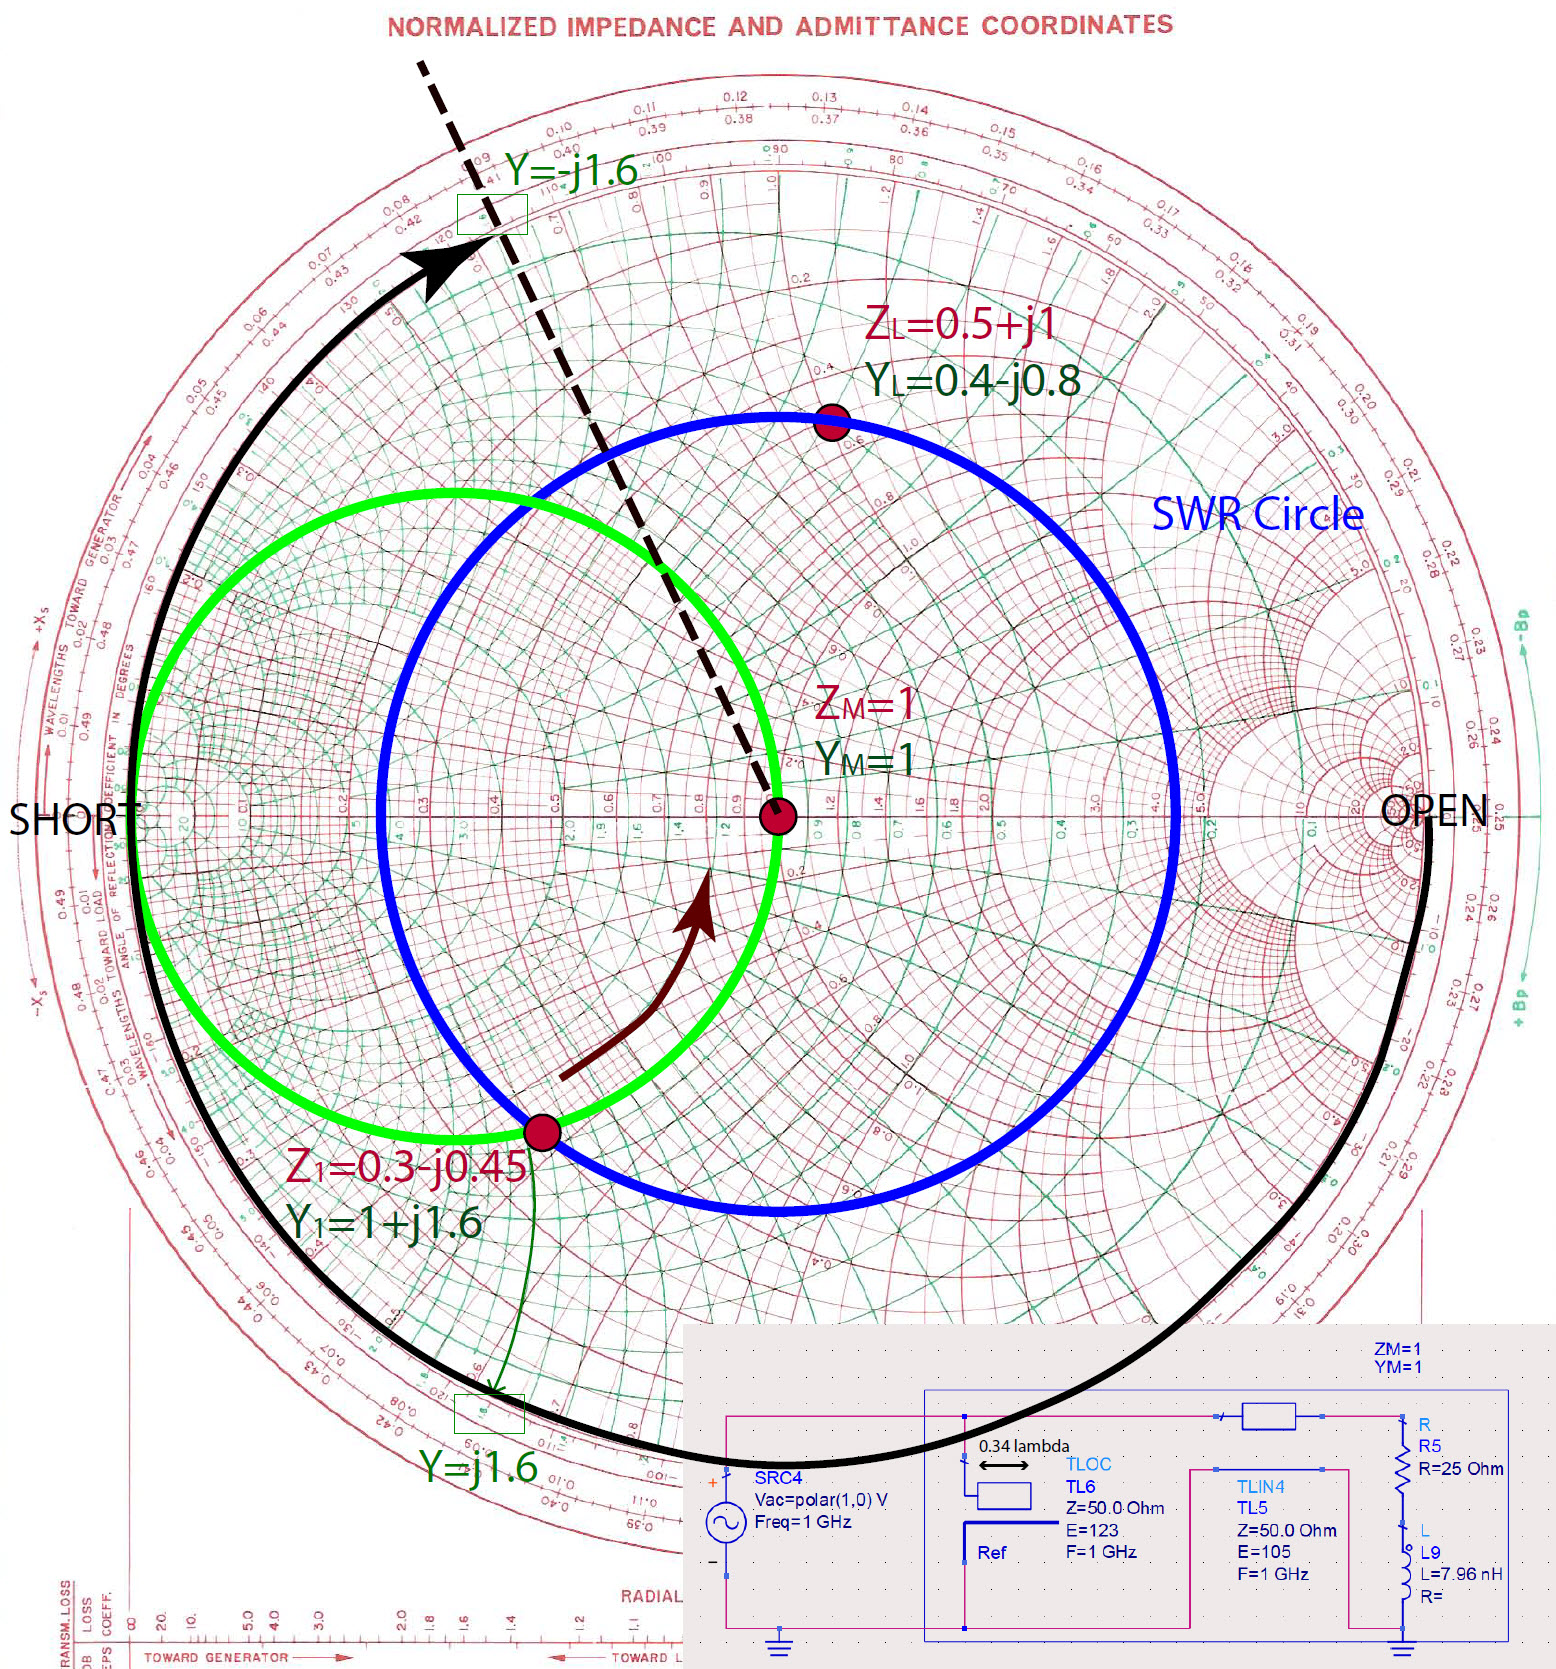
\includegraphics[scale=0.4]{../jpg/MatchTL.jpg}
\end{center}
\caption{Transmission-line impedance matching circuit.}
\label{fig:TransLineImpM}
\end{figure}


\section{Design of lumped-element impedance matching circuits}

In lumped-element impedance matching, we use only capacitors and inductors. Fully lumped-impedance matching circuits are used at lower frequencies, where transmission lines are too long to be practical for matching. Note that when we are matching the load with lumped elements, there are no SWR circles on the Smith Chart, because we are not using transmission lines.

Graphically, there are several different lumped-element impedance matching circuits that we can make for a specific impedance. For example,for impedance $Z_L=25+j50 \Omega$, there are four different 2-element circuits that we can make, as shown in Figure \ref{fig:LumpedVariety}. In the next paragraph we will use the orange path on the Smith Chart, with intermediate impedance $Z_2$.



\begin{figure}[htbp]
\begin{center}
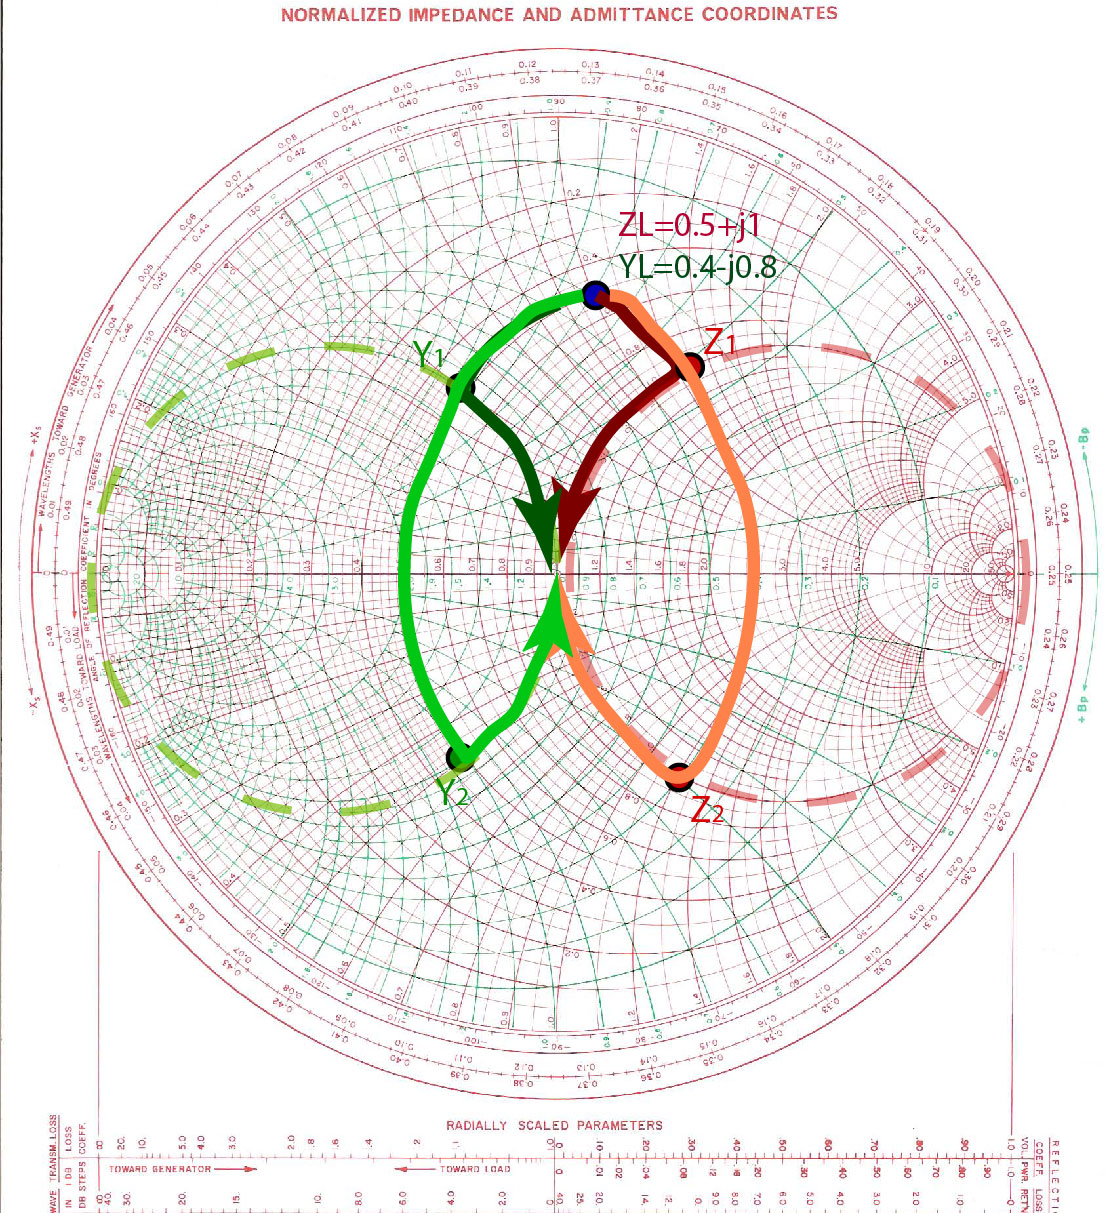
\includegraphics[scale=0.4]{../jpg/LumpedVariety-01.jpg}
\end{center}
\caption{A variety of lumped-element impedance matching circuits for impedance $Z_L=25+j50 \Omega$.}
\label{fig:LumpedVariety}
\end{figure}



We again start from the load impedance  $Z_L=25+j 100 \Omega$, and we normalize it to the $50 \Omega$ to get $\bar{Z}_L=0.5+j1$. The equivalent admittance of this impedance is $\bar{Y}_L=0.4-j0.8$. We identify the position of this impedance on the Smith Chart. Figure \ref{fig:LumpedImpM1} shows the green admittance line we follow to impedance $\bar{Z}_1=1-j1.2$. The equivalent admittance of this impedance is   $\bar{Y}_1=0.4+j0.5$. The green admittance line shows that we have to add $\bar{Y}_{add}=+j1.3$ to the load admittance $\bar{Y}_L=0.4-j0.8$ to get the total admittance of $\bar{Y}_1=0.4+j0.5$. $\bar{Y}_L+\bar{Y}_{add}=\bar{Y}_1$. Since we are adding two admittances, the elements have to be in parallel. Because the added admittance is positive, the added element is a capacitor, as shown in Figure \ref{fig:LumpedImpM1}. To find the capacitance of the capacitance we need to add in parallel, we first have to re-normalize the additional admittance $\bar{Y}_{add}$ by multiplying it with the $0.02$Si. The admittance of a capacitor is $j \omega C$ has to be equal to this added admittance. $2 \pi f C = 1.3* 0.02$. From this equation we find that the capacitance is $C \approx 4.1$pF. 
 


\begin{figure}[htbp]
\begin{center}
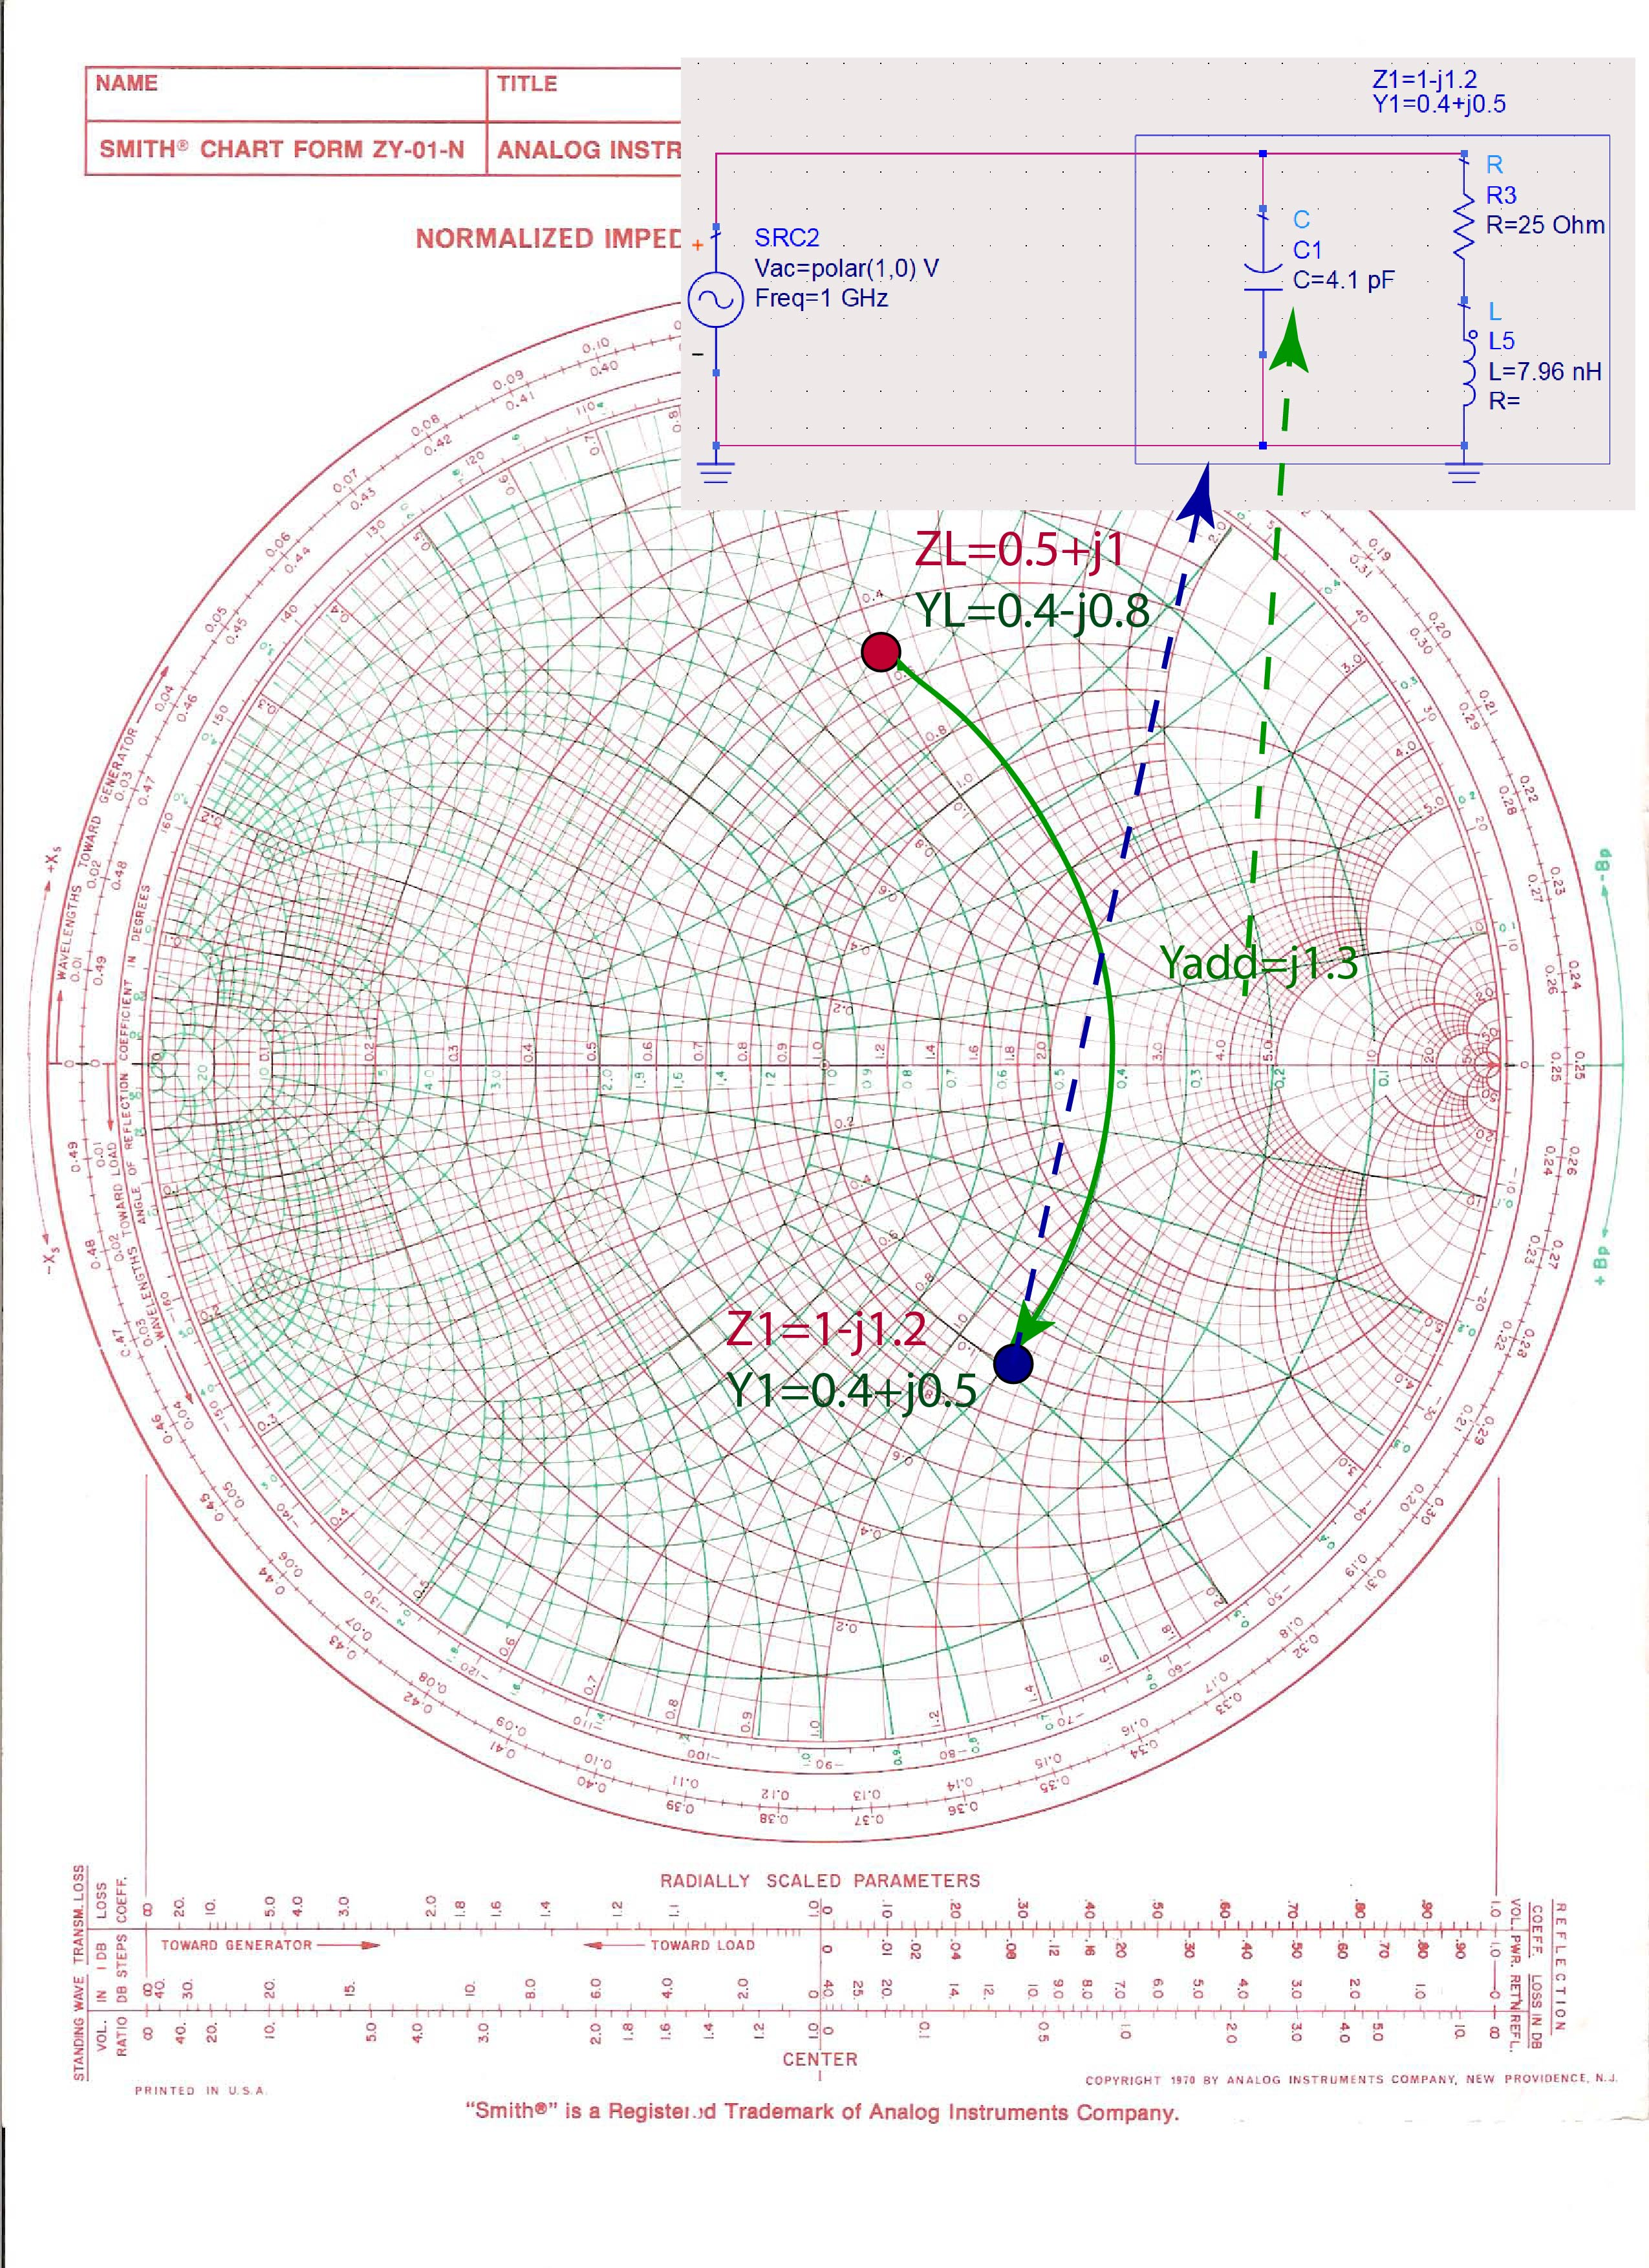
\includegraphics[scale=0.4]{../jpg/LumpedMatch1.jpg}
\end{center}
\caption{Adding an element in parallel to load impedance to get the equivalent real part of the impedance equal to one.}
\label{fig:LumpedImpM1}
\end{figure}


When we add $4.1$pF capacitor in parallel with the load $\bar{Z}_L=0.5+j1$, the total impedance of the two elements in parallel is $\bar{Z}_1=1-j1.2$.The real part of this impedance is already $50\Omega$. The final step is to remove the reactive part of the impedance by adding an additional impedance of $\bar{Z}_{add}=j1.2$, as shown in Figure \ref{fig:LumpedImpM3}. The total impedance is then $\bar{Z}_M=\bar{Z}_1+\bar{Z}_{add}=1$. Since we are adding two impedances, the elements must be in series. Because the added impedance is positive, it must be an inductor. To find the inductance of the inductor, $\bar{Z}_{add} 50=\omega L$. From this equation we get that the inductance is $L \approx 9.86 $nH.



\begin{figure}[htbp]
\begin{center}
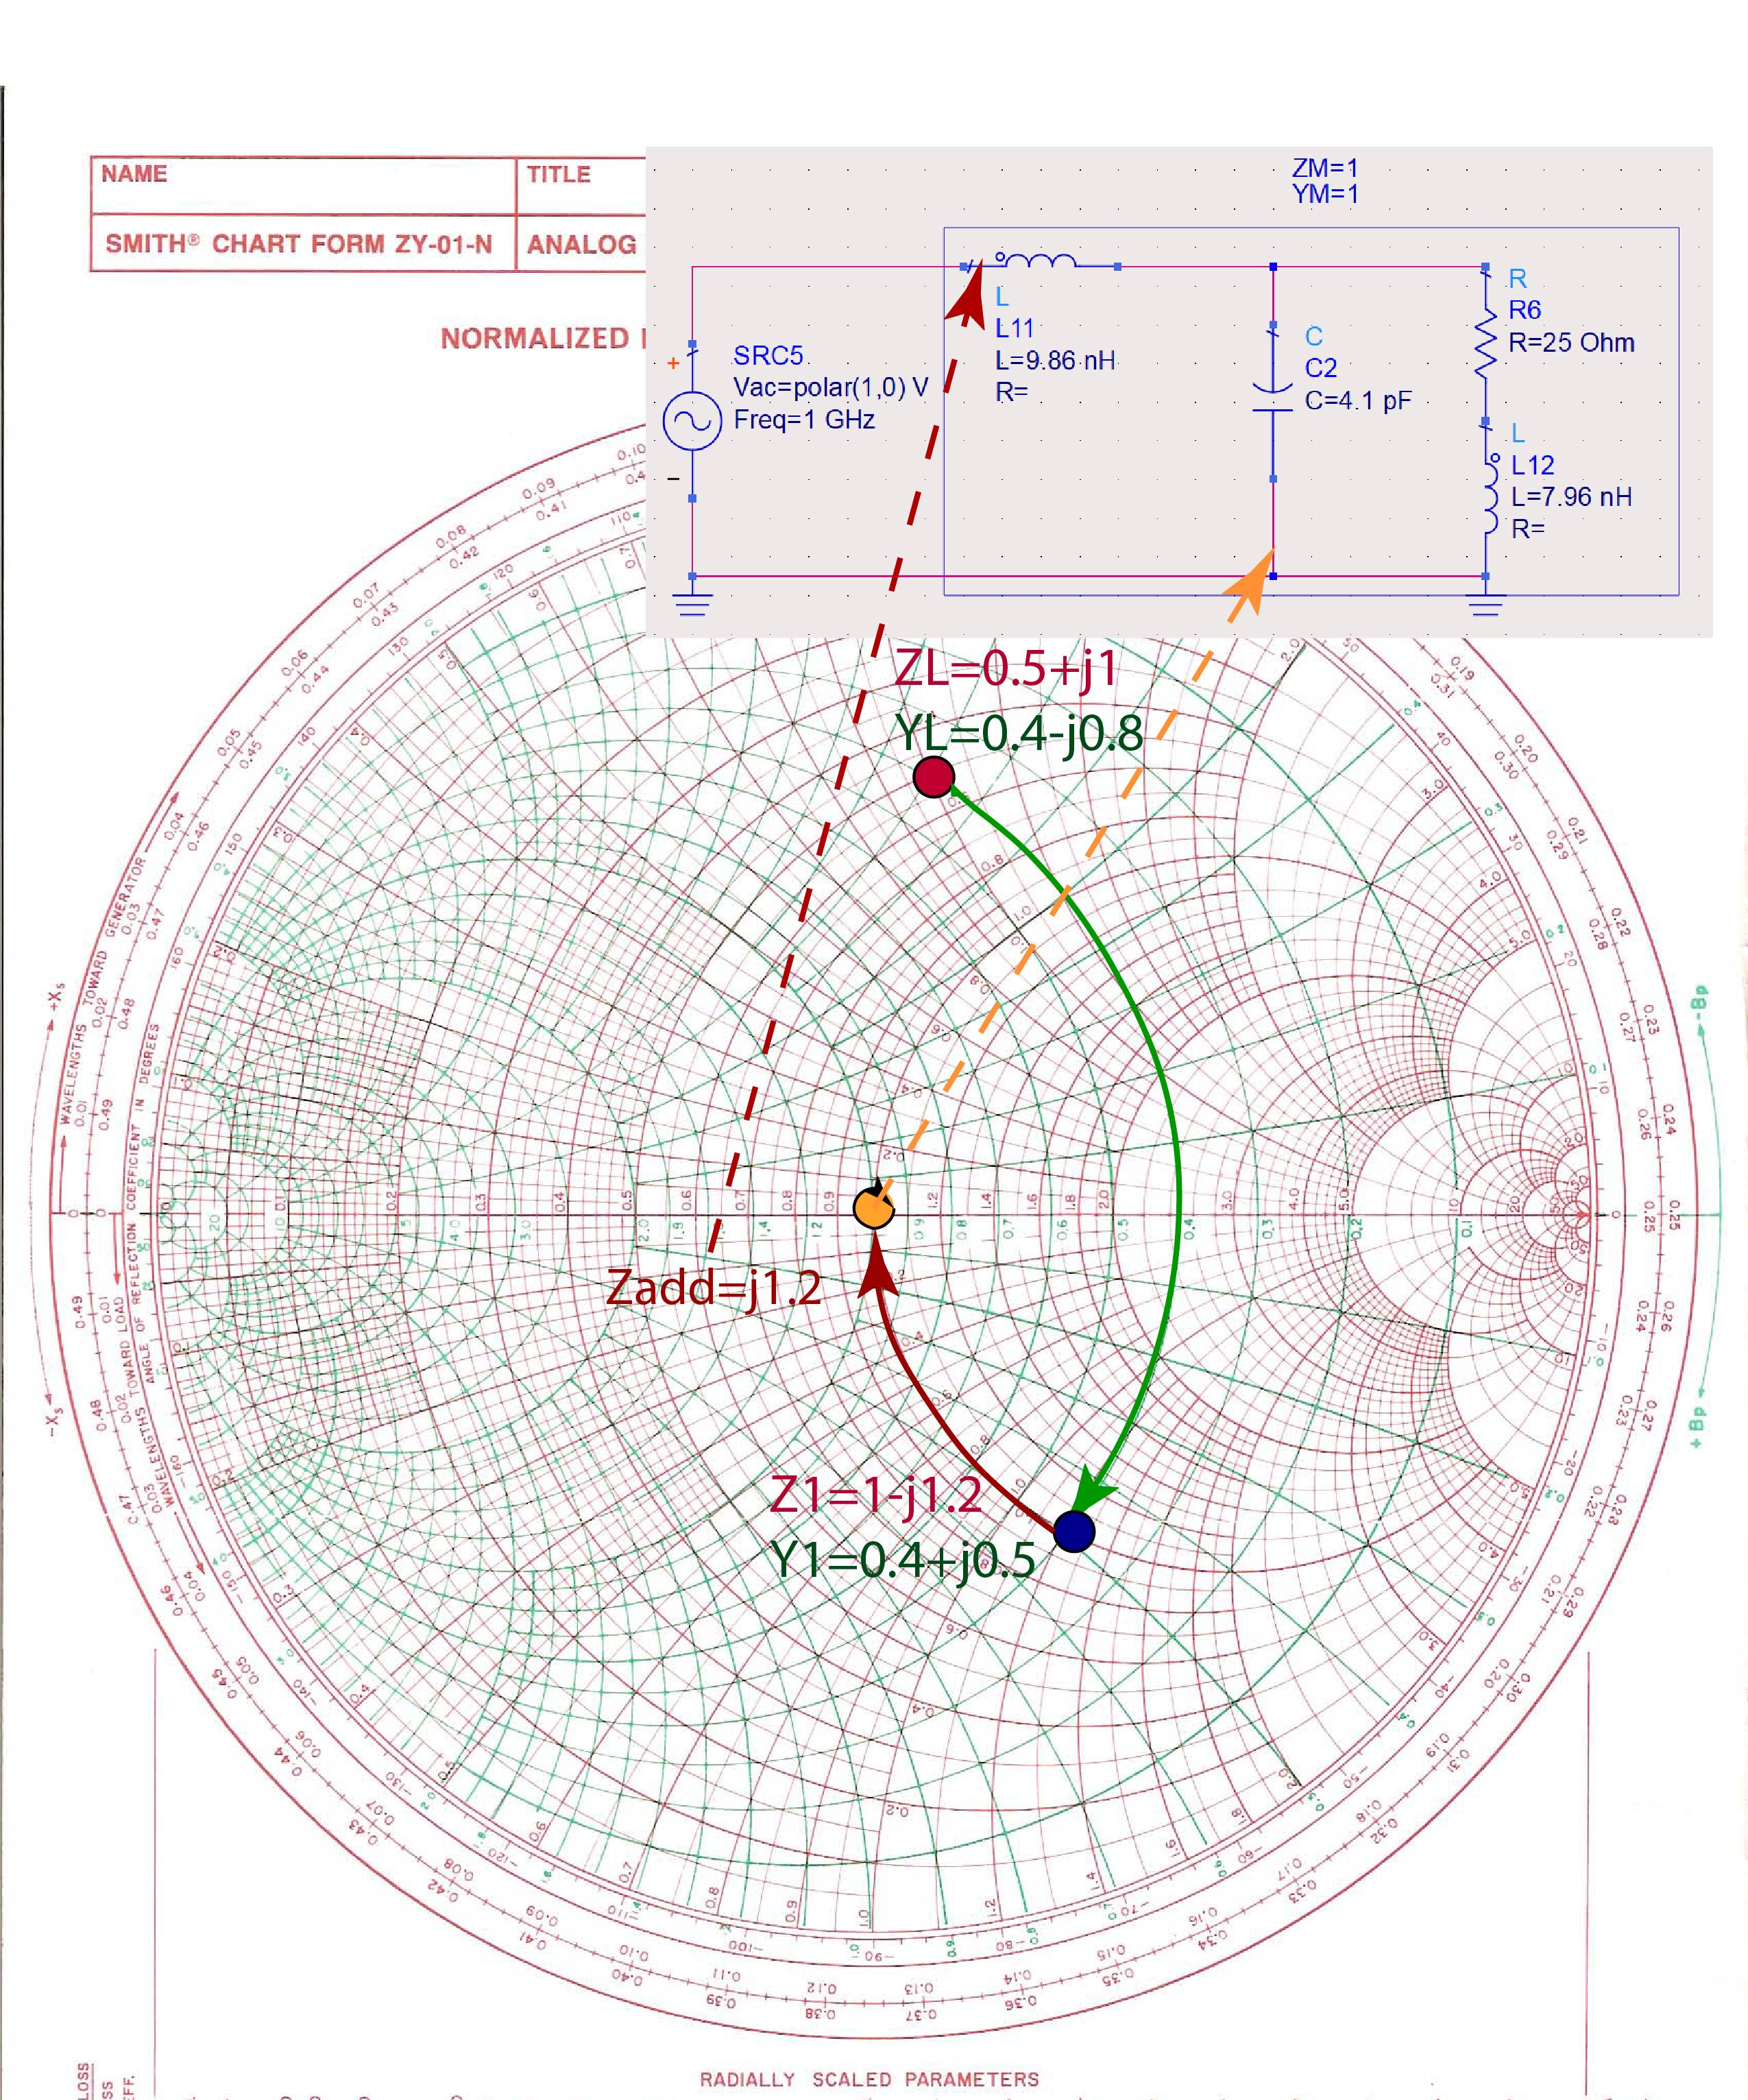
\includegraphics[scale=0.4]{../jpg/LumpedMatch3-01.jpg}
\end{center}
\caption{Finalized lumped-element impedance-matching circuit.}
\label{fig:LumpedImpM3}
\end{figure}

\end{document} 
